\documentclass{layout/layout}%
\usepackage{lastpage}%
\usepackage{pdfpages}%
\usepackage[]{algorithm2e}
\usepackage[round]{natbib}
\usepackage{amsfonts}
\usepackage{mathtools}

% Flowchart
\usepackage{tikz}
\usetikzlibrary{shapes,positioning}



\newcommand{\subtag}[1]{\tag{\theparentequation#1}}

\DeclareMathOperator*{\argmax}{arg\,max}
\DeclareMathOperator*{\argmin}{arg\,min}

%
\renewcommand{\deg}{\si{\degree}\xspace}%
\newcommand\ReportYear{2021}%
\newcommand\ReportMonthName{March}%
%
\newcolumntype{b}{X}
\newcolumntype{s}{>{\hsize=.5\hsize}X}

\begin{document}%
\normalsize%
\frontmatter%
\title{Strategic Asset Allocation}%
\subtitle{Estimation, Optimization, Visualization}%
\author{Juraj Hledik}%
\subject{\ReportMonthName \  \ReportYear}%
\coverimage{figures/cover7.jpg}%
\definecolor{title}{HTML}{4884d6}%
\makecover%
\chapter*{Preface}
\addcontentsline{toc}{chapter}{Preface}

This report summarizes my suggestions regarding the process of strategic asset allocation within the National Bank of Slovakia. I have worked on this project during spring and summer of 2022 as a full-time member of the NBS's research department. In case of inquiries regarding the code or the documentation, please contact me at hledik.juraj@gmail.com
\begin{flushright}
{\makeatletter\itshape
    \@author \\
    %Vienna, \ReportMonthName, \ReportYear
\makeatother}
\end{flushright}
%
\tableofcontents%
\listoffigures%
\listoftables%
\mainmatter%
\chapter*{Introduction}
\label{chapter:introduction}

This report summarizes key concepts and ideas related to NBS's strategic asset allocation. As is common in the literature on portfolio allocation, we shall divide the process of creating an optimal portfolio according to investor preferences into two consecutive steps:
\begin{itemize}
	\item Estimation of future asset returns.
	\item Solving a portfolio optimization problem given the prediction from step 1.
\end{itemize}
To make our approach as modular as possible, we will threat these two tasks independently, allowing the future users of our pipeline to use them separately. In other words, if someone were to have their own prediction regarding future returns, they are welcome to plug this prediction into our optimization module and use our framework solely for finding an efficient portfolio allocation. Likewise, if one were to have their own portfolio optimization algorithm prepared, they are welcome to use the first part of our approach only (generate future return predictions using our framework) and then plug the predicted returns into their own optimization algorithm. Keeping these two concepts independent therefore gives us further flexibility and freedom in model choice.

There are 4 chapters in this report. Chapter 1 describes estimation of future asset returns from historical data. Chapter 2 then uses this prediction to formulate a modular and flexible portfolio allocation strategy. Finally, Chapter 3 summarizes the graphical user interface used to achieve tasks from previous chapters, describes the data pipeline structure and other technical details.


% Reason

% Aim

% Structure
%
\chapter{Return estimation}

This chapter summarizes the first step in strategic asset allocation - estimation of future returns' probability density function. We will cover everything from data import to the drawing/simulation of future returns from an estimated distribution.

\section{The data}

The data available at our disposal consist of daily returns dating back almost two decades for eight representative asset classes. In the spirit of our modular approach, the investor is able to input their own return observations and preferred asset classes into our framework. Throughout this chapter, however, we will assume a given set of eight asset classes and explain our future return estimation mechanics on this particular asset class set.

The assets used in our analysis contain indices following the prices of gold, US Treasury bonds, a specific ASW portfolio, world equity, Chinese government bonds, US Inflation-linked government bonds, Mortgage-backed securities and emerging markets. These are all summarized in Table \ref{tab:return_estimation:asset_classes} and form our basic 8 available asset classes.
\begin{table}[h]
	\centering
	\begin{tabularx}{0.9\linewidth}{rX}
		Asset class & Relevant index\\
		\toprule
		\textbf{Gold} & Gold XAU/EUR Rate FX Unhdg.
		 \\
		\textbf{US} & 1-5 Year US Govt (ICE) FX Unhdg.
		 \\
		\textbf{ASW} & 1-5 Year Global Non-Sov (ICE) IR hdg. IRS
		 \\
		\textbf{Stocks} & World Equity (MSCI) FX Unhdg.
		\\
		\textbf{China} & 1-3 Year China Govt (ICE) FX Unhdg.
		\\
		\textbf{InflBonds} & US Inflation-Linked Govt (ICE) FX Hdg.
		\\
		\textbf{MBS} & US MBS (ICE) FX Hdg.
		 \\
		\textbf{EM} & EM global IG Govt (JPM) FX Hdg.
		 \\
		
		\bottomrule
	\end{tabularx}
	\caption{Asset classes.}
	\label{tab:return_estimation:asset_classes}
\end{table}

\section{The return simulation process}

Following consecutive steps are part of the return estimation process:

\begin{table}[h]
	\centering
	\begin{tabularx}{0.9\linewidth}{lXX}
		Parameter & Description & Default value\\
		\toprule
		\textbf{N\_simulation} & Number of returns that are being simulated. From these, the final returns are drawn uniformly randomly, depending on sample size. Therefore must be greater than $\max\left[\text{sample\_sizes}\right]$. & 1 000 000
		\\
		\textbf{sample\_sizes} & Sample sizes for which future returns are simulated. & (100, 500, 1000, 2000, 5000, 10000, 50000, 100000) 
		\\
		\textbf{maturities} & Maturities for which future returns are simulated.& (1,3,6,12,60) 
		\\
		\textbf{frequency} & Frequency to which daily historical returns are being transformed first. & monthly
		\\
		\textbf{selected\_copula\_types} & Selection of available copula families that are allowed to be used within the model selection procedure. & all copulas available in the VineCopula package for R
		\\
		\bottomrule& 
	\end{tabularx}
	\caption{User parameters used in return estimation and simulation.}
	\label{tab:return_estimation:user_parameters}
\end{table} 
\begin{enumerate}
	\item User parameters specified. These include the sample size of simulated future return distribution, maturity of said returns, frequency of historical returns used in such estimation etc. For a full list of relevant user parameters, see Table \ref{tab:return_estimation:user_parameters}.
	\item Imported daily data.
	\item Created a new dataset with observation frequency chosen by the user - daily, weekly, monthly or yearly. Data saved in a relevant folder.
	\item Fit each asset class with both Gaussian as well as Pearson type VII distribution.
	\item Transform each asset class into a $[0,1]$ uniformly distributed variable using the distributional assumption of a Pearson type VII distribution.
	\item Fit the copula to the uniformly distributed marginal data, drawing from the allowed copula families selected by the user.
	\item Use the fitted model to generate $N\_simulation$ observations of simulated returns / draw them from the estimated distibution. Also draw the same number of returns from multidimensional Gaussian distribution.
	\item Plot pairwise correlations of the simulated Pearson + Copula vs. Gaussian returns vs. historical data to allow for a visual comparison.
	\item Compute the Cramer and Kolmogorov-Smirnov tests on distributional equality to evaluate the similarity of simulated return distribution to the original distribution.
	\item Use the simulated returns to create datasets with different maturities and sample sizes - daily, weekly, monthly and yearly. Save them in a pre-specified directory structure together with the relevant estimated copula structure.
\end{enumerate}

This process can also be schematically viewed as an algorithm in Algorithm \ref{alg:return_estimation}. Several steps in this procedure however warrant further clarification and details, which we shall focus on in the following paragraphs.

\begin{algorithm}[!htb]
	\KwData{historical returns}
	\KwIn{N\_simulation, sample sizes, maturities, frequency, copula\_types}
	\KwResult{simulated returns}
	import historical return data\;
	\eIf{frequency=="daily"}{
		no aggregation;
	}{
		\eIf{frequency=="weekly"}{
			aggregate to weekly returns\;
		}{
			\If{frequency=="monthly"}{
				aggregate to monthly returns\;
			}
		}
	}
	set custom asset names\;
	create directory structure\;
	save aggregated	data\;
	\ForEach{asset class}{
		estimate the Pearson and Gaussian distribution parameters\;
		generate simulated returns from Pearson and Gaussian distribution\;
		plot marginal historical return distribution with Pearson and Gaussian fit\;
		transform asset class to a $[0,1]$ uniform distribution\;
	}
	fit a multivariate Gaussian distribution to the data;\
	fit the copula to the uniform data, drawing from allowed copula types\;
	plot historical vs. simulated returns in a pairwise correlation plot\;
	run a Cramer test on equality of distributions with the historical data for both models (Gaussian and copula)\;
	\ForEach{asset class}{
		run a Kolmogorov-Smirnov test of distributional equality with the historical data for both models\;
	}
	save results of Cramer and K-S tests\;
	\For{sample sizes}{
		\For{maturities}{
			store the simulated returns in the relevant path;\
			acording to the frequency, compute the p.a. returns and store them in the appropriate path\;			
		}
	}
	store the copula structure\;
	\caption{Return estimation and simulation.}
	\label{alg:return_estimation}
\end{algorithm}

The data on historical returns is stored as a \textit{historical\_daily\_returns.csv} file with columns corresponding to the different asset classes and rows corresponding to daily returns. Furthermore, we also use an input file called \textit{portfolio\_constraints.xlsx} which besides relevant default investor constraints also contains short versions of the respective asset class names.

In the first step, the returns are loaded into R, formatted as numeric values and transformed to a desired frequency chosen by the user. The transformation from daily observations to e.g. weekly observations is done by:
\begin{enumerate}
	\item adding 1 to each observation,
	\item multiplying the observations corresponding to a particular week,
	\item subtracting 1 from the result.
\end{enumerate}
The new dataframe is now taken as a baseline. We assign custom asset class names to all variables (taken from \textit{portfolio\_constraints.xlsx}) and save this dataset in an appropriate data folder (for directory structure of the project, refer to the technical summary at the end of this report).

In the second step, we estimate both the Pearson and Gaussian marginal distributions that are the best fits for our data. A one-dimensional Gaussian distribution has the following density function:

\begin{equation}
f(x)={\frac {1}{\sigma {\sqrt {2\pi }}}}e^{-{\frac {1}{2}}\left({\frac {x-\mu }{\sigma }}\right)^{2}}
\end{equation}

where $\mu$ is the expected value and $\sigma$ is the variance of the distribution. We compute these quantities from the sample for each asset class and hence obtain the desired Gaussian distribution parameters.

A Pearson type VII distribution density is slightly more complicated, with three parameters instead of two:


\begin{equation}
f(x\mid \lambda, \alpha, m)={\frac {1}{\alpha \operatorname {\mathrm {B} } \left(m-{\frac {1}{2}},{\frac {1}{2}}\right)}}\left[1+\left({\frac {x-\lambda }{\alpha }}\right)^{2}\right]^{-m}
\end{equation}

The benefits associated with this distribution mostly lie in its scalability with respect to its fourth moment - kurtosis. This freedom allows us to better approximate the historical returns not only in their mean and variance, but also in terms of their tails. This property is especially crucial if we are dealing with investor that places high importance on tail-relevant risk measures such as Value-at-Risk or expected shortfall. In light of such preferences, having a reliable way of predicting tail events is of utmost importance.

An alternative parameterization of the Pearson type VII distribution can be achieved by substituting $\alpha := \sigma\sqrt{2m-3}$. In such case, letting $m$ approach the infinity provides us with a well-known Gaussian distribution as the kurtosis approaches the value of 3. Assuming $m>5/2$ guarantees the existence of the distributions' first four moments. Another substitution of $\lambda=\mu, \alpha=\sqrt{\nu\sigma^2}, m=\frac{\nu+1}{2}$ then gives us the non-standardized Student's t distribution
\begin{equation}
f(x\mid \mu ,\sigma ^{2},\nu )={\frac {1}{{\sqrt {\nu \sigma ^{2}}}\,\operatorname {\mathrm {B} } \left({\frac {\nu }{2}},{\frac {1}{2}}\right)}}\left(1+{\frac {1}{\nu }}{\frac {(x-\mu )^{2}}{\sigma ^{2}}}\right)^{-{\frac {\nu +1}{2}}}
\end{equation}
After some basic algebraic computations, we can show that a random variable $X$ with this particular distribution has its first four moments given by the following formulae:
\begin{eqnarray}
	\text{E}[X] &=& \mu \\ 
	\text{Var}[X] &=& \sigma^2\frac{\nu}{\nu-2} \\
	\text{Skew}[X] &=& 0 \\
	\text{Kurt}[X] &=& \frac{3\nu-6}{\nu-4}
\end{eqnarray}
With this in mind, we can estimate parameters $\mu, \sigma$ and $\nu$ from the first four moments of historical returns simply by letting these expressions be equal to sample-specific moments. With the distribution successfully parameterized, we can easily draw an arbitrary number of simulated returns from the estimated distribution.


\begin{figure}[!htb]
	\begin{subfigure}{.49\textwidth}
		\centering
		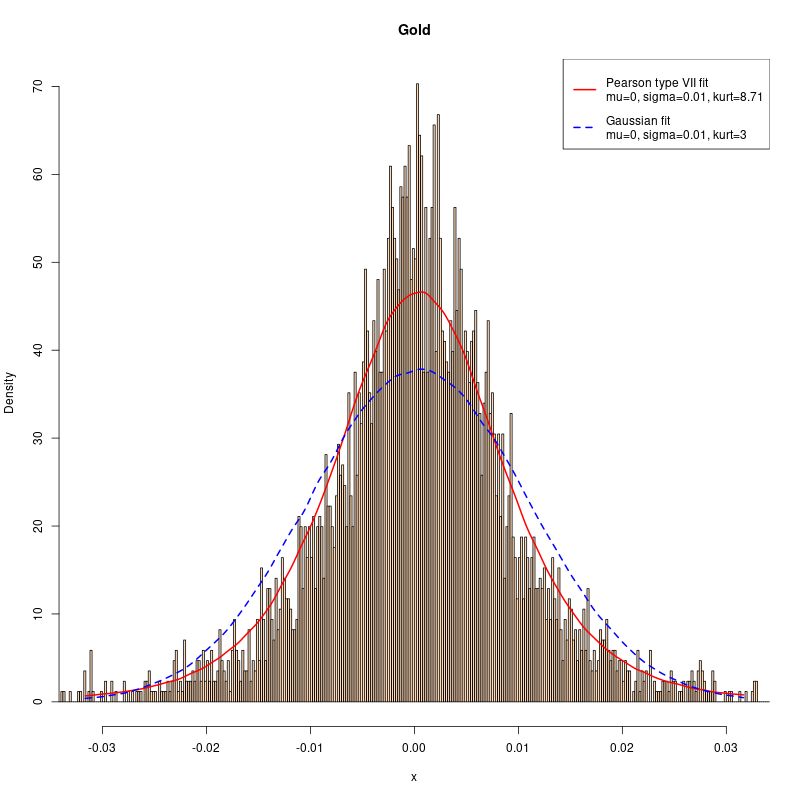
\includegraphics[width=\textwidth]{\detokenize{figures/marginal_distributions/Gold}}
		\caption{Gold}	
	\end{subfigure}
	\begin{subfigure}{.49\textwidth}
		\centering
		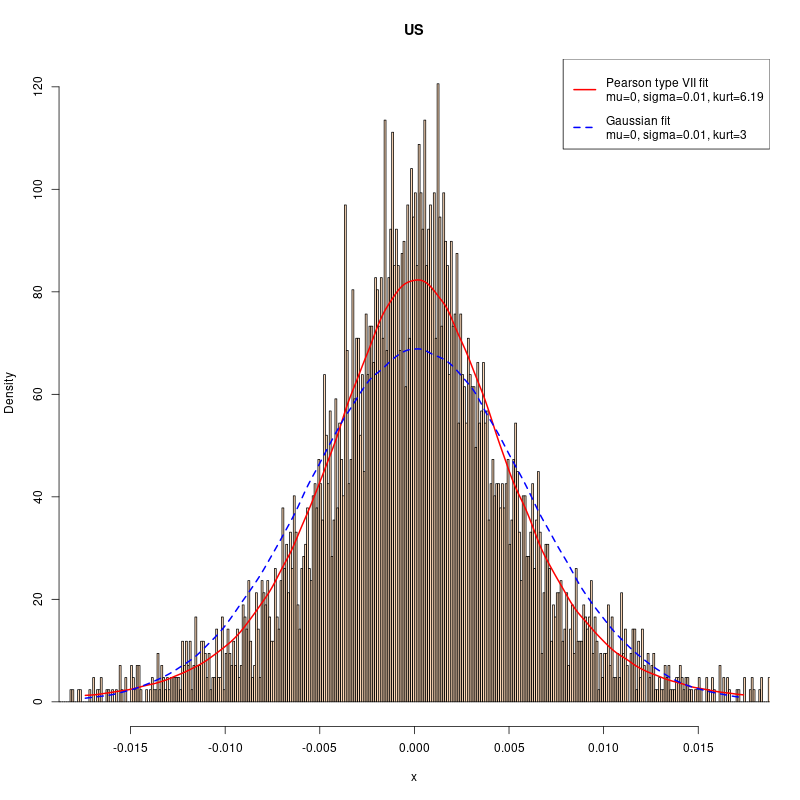
\includegraphics[width=\textwidth]{\detokenize{figures/marginal_distributions/US}}
		\caption{US Government Bonds}
	\end{subfigure}\\
	\begin{subfigure}{.49\textwidth}
		\centering
		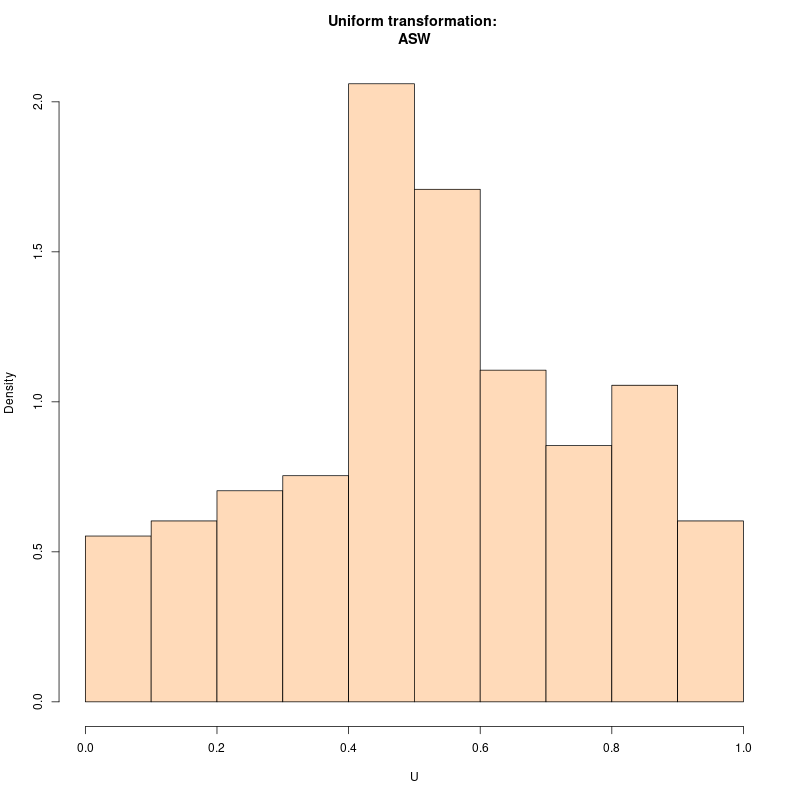
\includegraphics[width=\textwidth]{\detokenize{figures/marginal_distributions/ASW}}
		\caption{ASW portfolio}
	\end{subfigure}
	\begin{subfigure}{.49\textwidth}
		\centering
		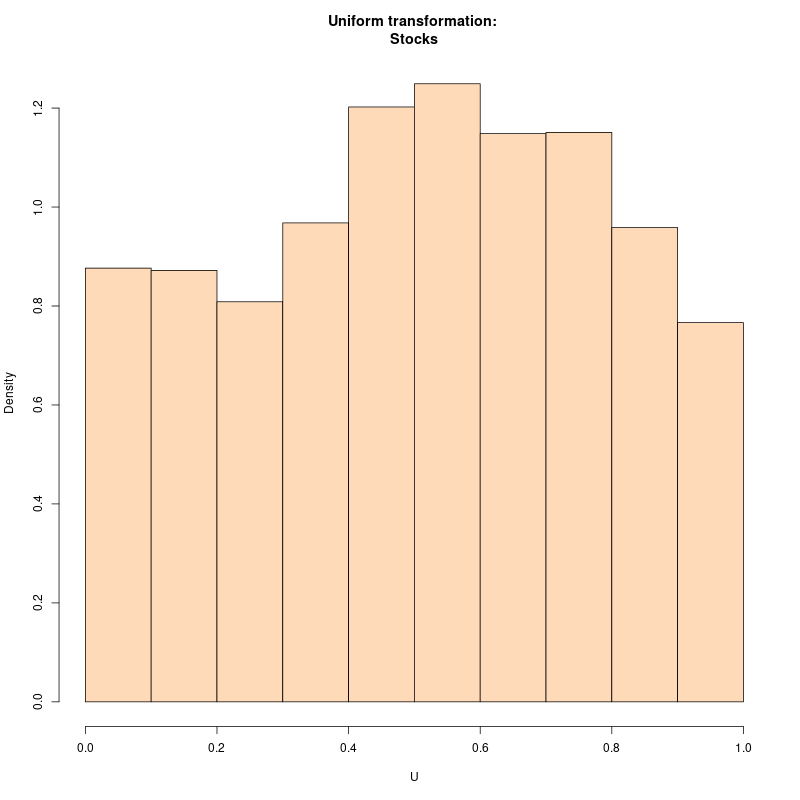
\includegraphics[width=\textwidth]{\detokenize{figures/marginal_distributions/Stocks}}
		\caption{World Equity}
	\end{subfigure}
	\caption{Historical returns, density approximated with a Gaussian and Pearson distributions. Part 1/2.}
	\label{fig:return_estimation:marginal_distributions_1}
\end{figure}
\begin{figure}[!htb]
	\begin{subfigure}{.49\textwidth}
		\centering
		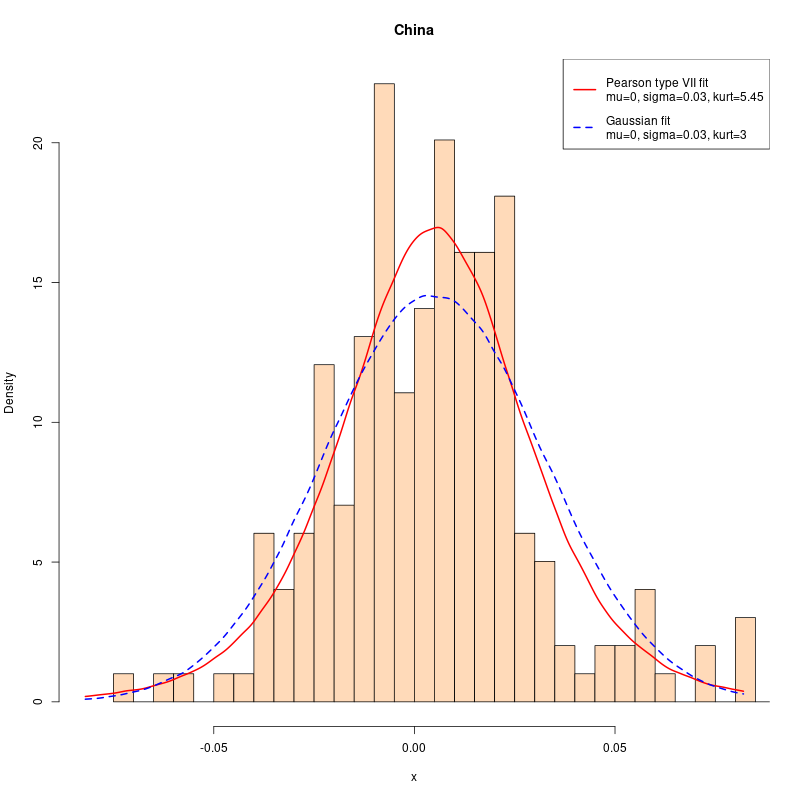
\includegraphics[width=\textwidth]{\detokenize{figures/marginal_distributions/China}}
		\caption{China Government Bonds}
	\end{subfigure}
	\begin{subfigure}{.49\textwidth}
		\centering
		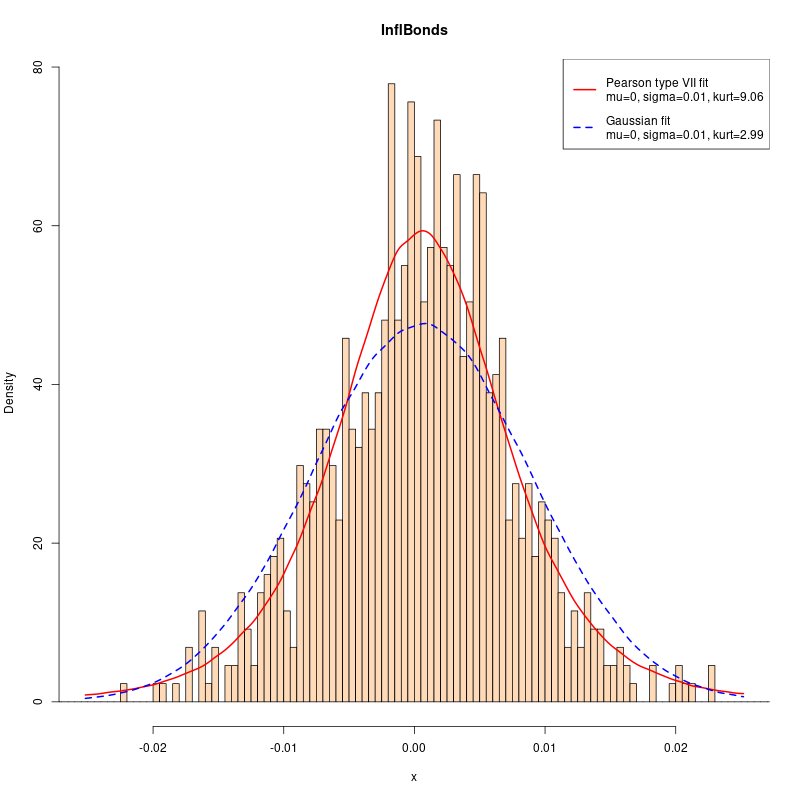
\includegraphics[width=\textwidth]{\detokenize{figures/marginal_distributions/InflBonds}}
		\caption{US Inflation-linked Government Bonds}
	\end{subfigure}\\
	\begin{subfigure}{.49\textwidth}
		\centering
		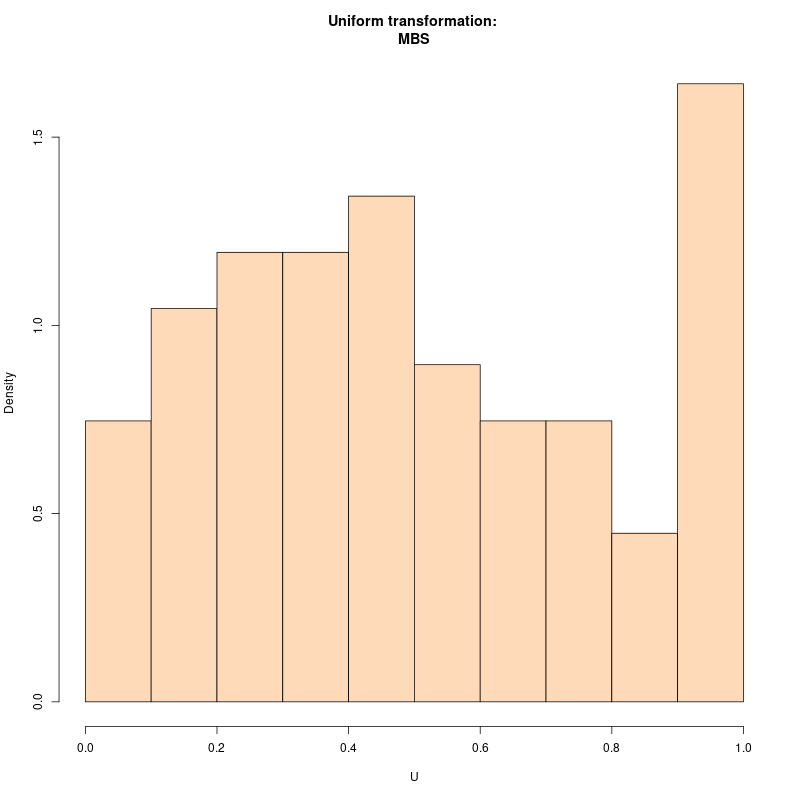
\includegraphics[width=\textwidth]{\detokenize{figures/marginal_distributions/MBS}}
		\caption{US Mortgage-backed Securities}
	\end{subfigure}
	\begin{subfigure}{.49\textwidth}
		\centering
		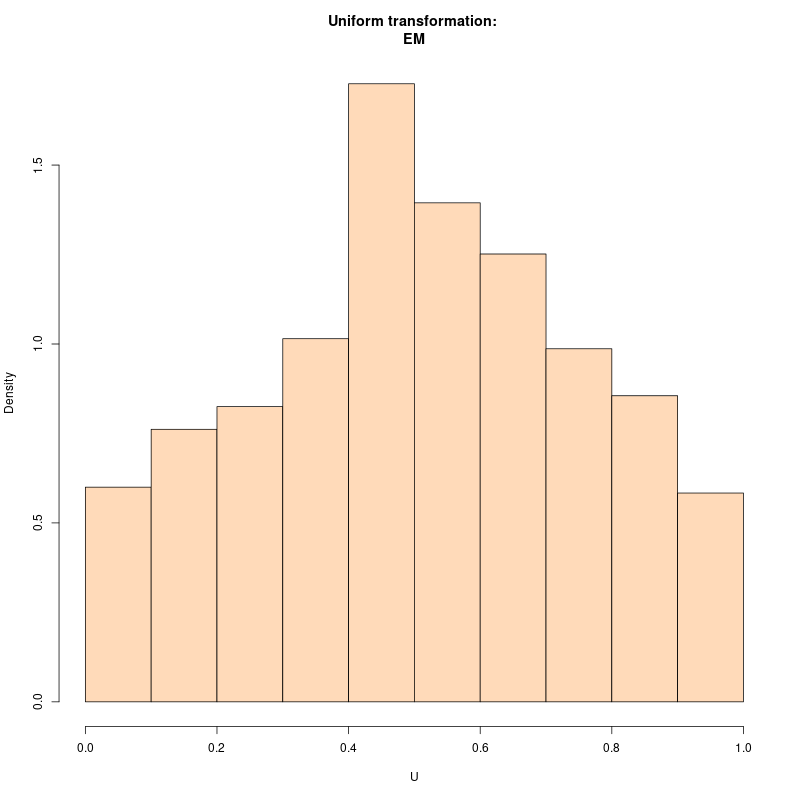
\includegraphics[width=\textwidth]{\detokenize{figures/marginal_distributions/EM}}
		\caption{Emerging markets}
	\end{subfigure}
	\caption{Historical returns, density approximated with a Gaussian and Pearson distributions. Part 2/2}
	\label{fig:return_estimation:marginal_distributions_2}
\end{figure}


Figures \ref{fig:return_estimation:marginal_distributions_1} and \ref{fig:return_estimation:marginal_distributions_2} show the relevant fit for both the Gaussian as well as the Pearson (non-standardized Student's t) distribution. The blue line corresponds to the Gaussian distribution, while the red line shows the fit of the Pearson type VII distribution.

We see that - in line with our expectations - using a distribution with variable kurtosis parameter allows for a tighter fit, especially in asset classes with fatter tails. But even though a brief visual examination is a great tool, we will also look into this goodness of fit more formally with proper statistical tests.

Before doing so, however, we shall focus on estimating the whole multidimensional distribution, not just the marginals. Again, we will do this for both the Pearson as well as the Gaussian distribution. In the former case, we shall use vine copulas for mutual pairwise dependencies, while in the latter case, we would estimate parameters of multivariate Gaussian distribution directly.

Starting with the Pearson distribution, we first transform each asset class into a $[0,1]$ uniform variable which is a necessary first step for fitting a copula model. The process is simply achieved by taking the estimated Pearson distribution function from the previous step and evaluating it at the respective historical return data points. In other words, if the random variable $X$ corresponds to our historical returns with assumed Pearson type VII cumulative distribution function $F(x)$, then the new random variable obtained by:
\begin{equation}
	U = F(X)
\end{equation}
is uniformly distributed at its domain $[0,1]$.
Transforming all asset classes this way shrinks our 8-dimensional real space into an 8-dimensional unit cube $[0,1]^8$. 

With the data transformed to a unit cube, we take advantage of the R package "Vine Copula", see \citep{2021VineCopulaPackage}. This package contains functions and routines focused on estimation and model selection of multivariate pairwise copulas also called the vine copulas. The function "\textit{RVineStructureSelect}" allows us to use its heuristical model-selection algorithm which automatically chooses and estimates the best pairwise copula model for our dataset given our choice of allowed copula families. Further details regarding the algorithm and the package in general can be found in \citep{2013Dissmann}.

Once the model is fitted, we draw N\_simulation returns from their estimated joint distribution. We follow the same approach with the multivariate Gaussian distribution, only instead of pairwise copulas, we simply use the maximum likelihood approach to estimate the distribution's vector of mean returns $\mu$ and the variance-covariance matrix $\Sigma$.

At this point, we have three sets of returns at our disposal: historical returns, Pearson type VII distributed returns with their mutual dependency given by pairwise copulas and a return set with multivariate Gaussian distribution. Pairwise dependency plot of these 3 classes of returns can be found in Figure \ref{fig:return_estimation:correlations}.

\begin{figure}[!htb]
	\centering
	\begin{subfigure}{.75\columnwidth}
		\centering
		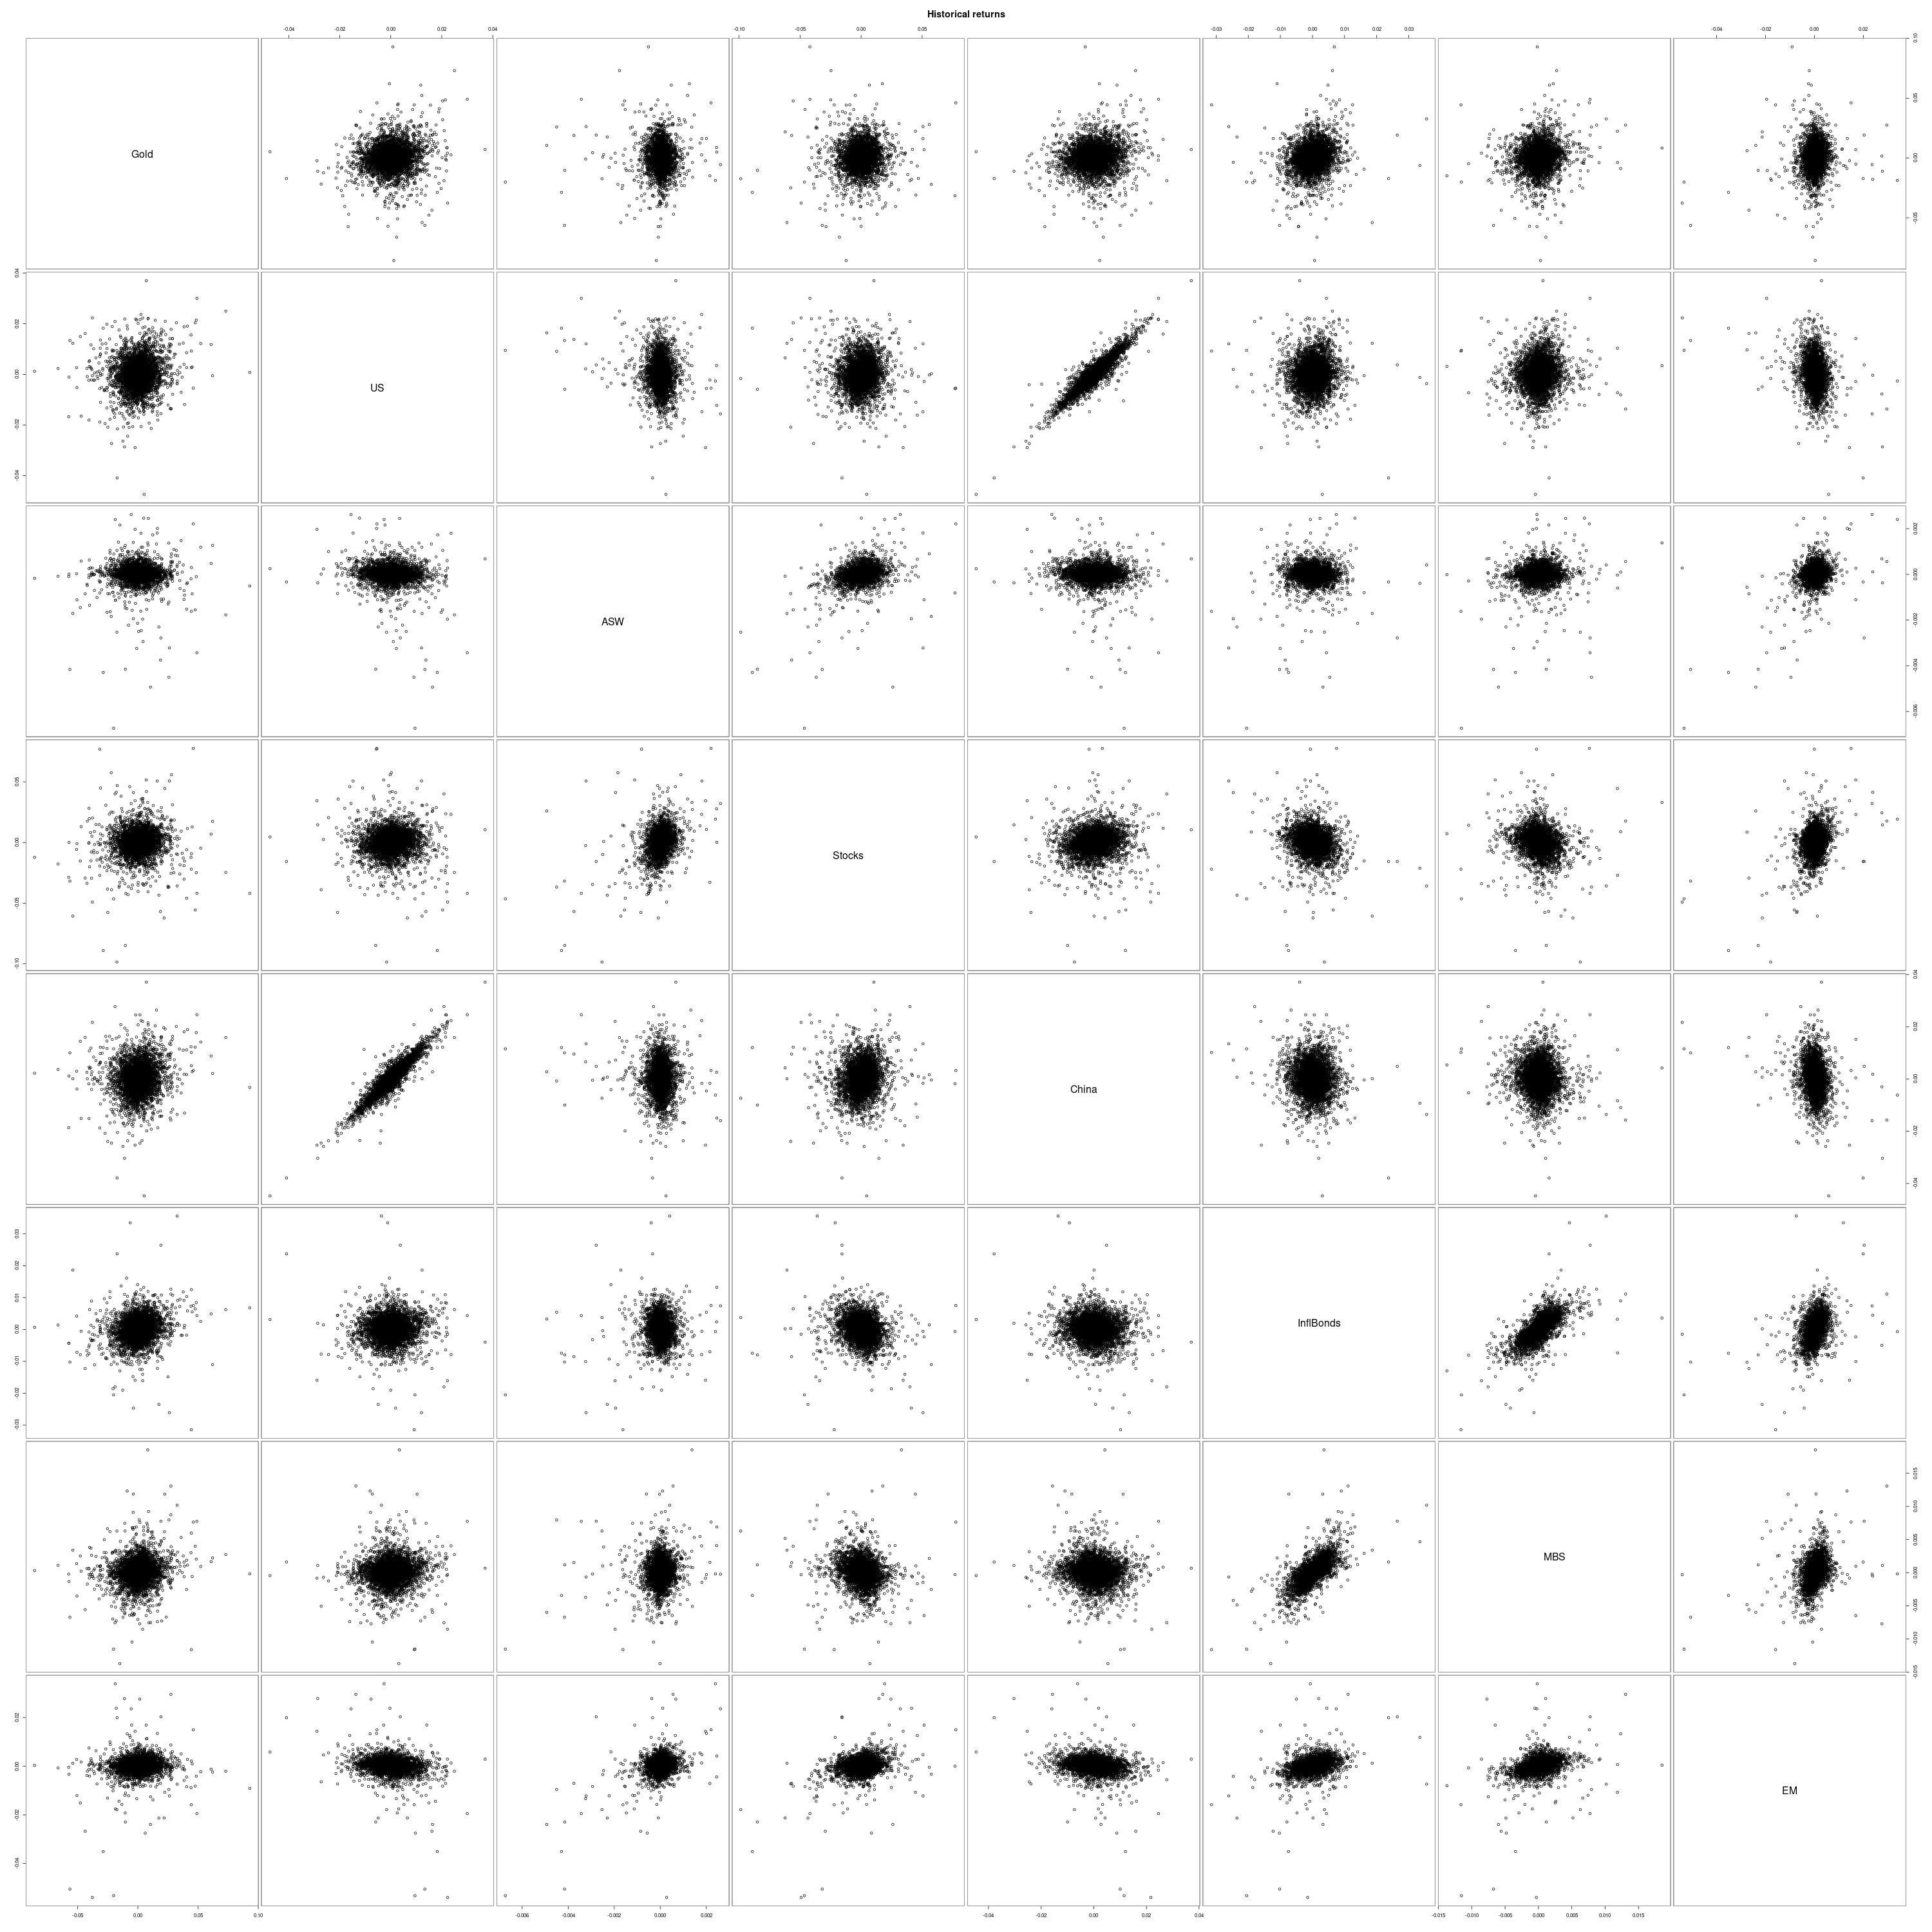
\includegraphics[width=\textwidth]{\detokenize{figures/correlations/Historical_Returns}}
		\caption{Historical returns}
	\end{subfigure}\\
	\begin{subfigure}{.75\columnwidth}
		\centering
		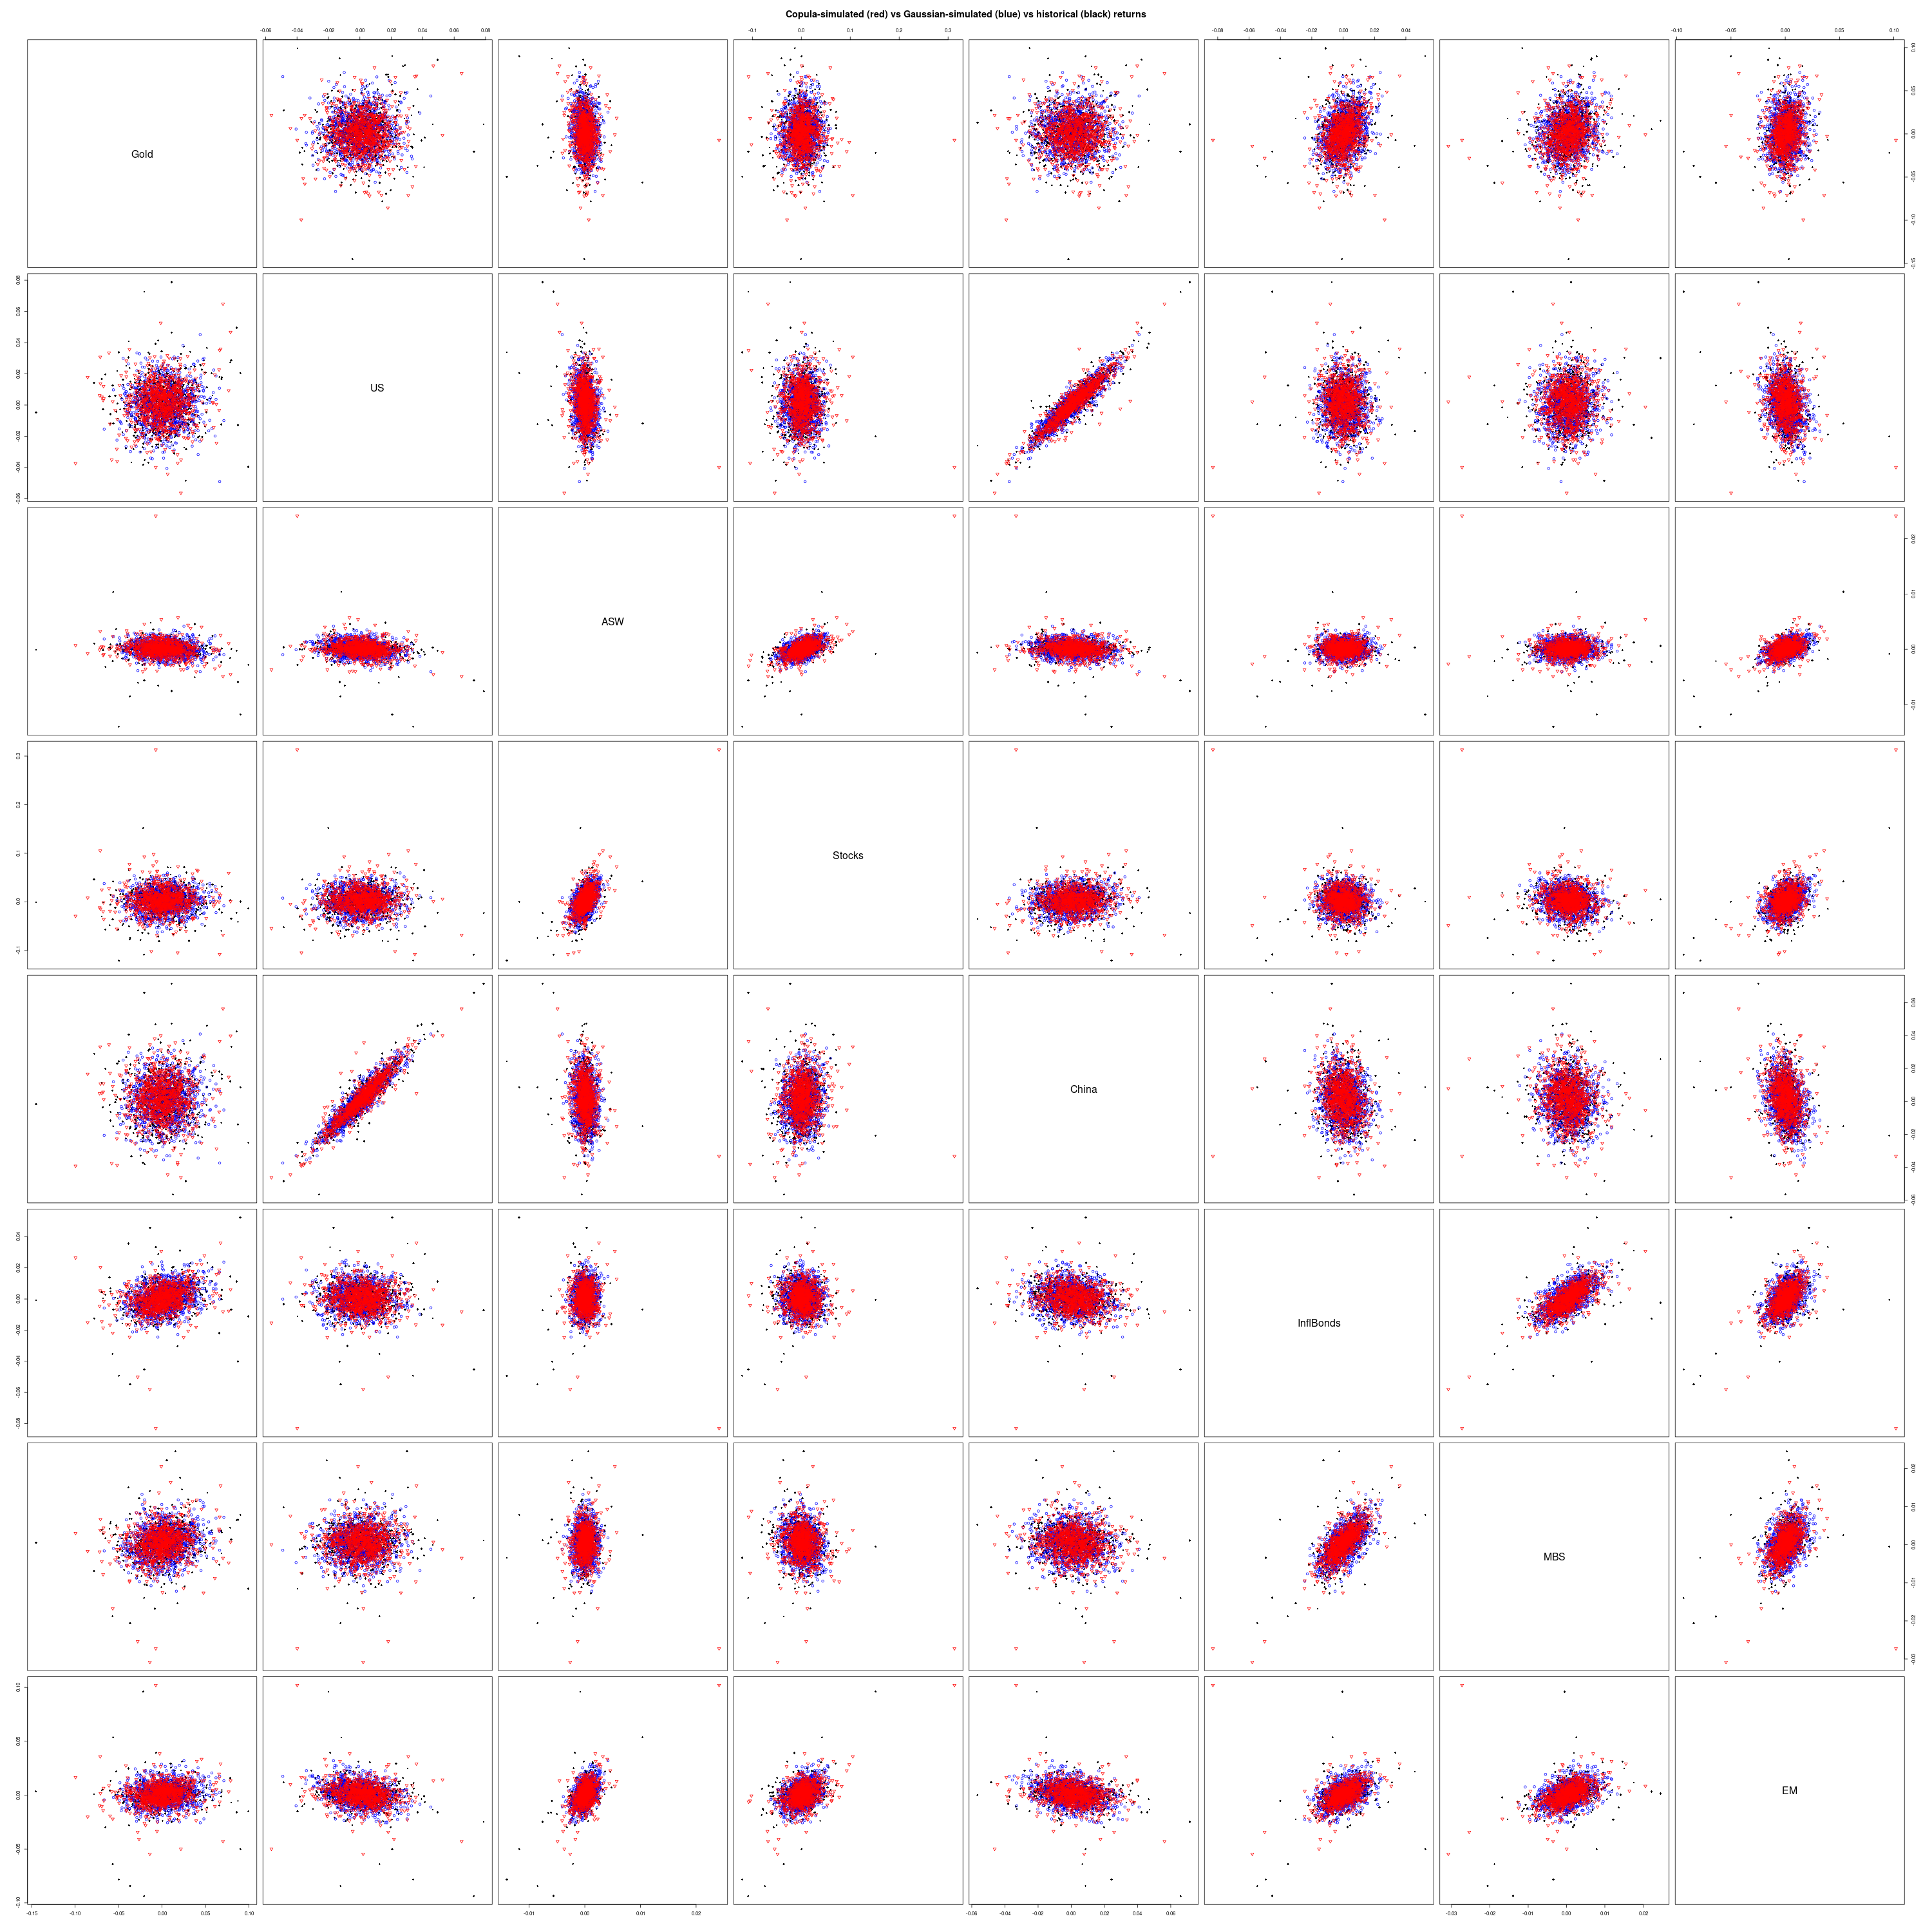
\includegraphics[width=\textwidth]{\detokenize{figures/correlations/Historical_vs_Gaussian_and_Pearson_returns3000}}
		\caption{Historical returns (black), Gaussian-distributed returns (blue) and Pearson-distributed returns(red)}
	\end{subfigure}
	\caption{Historical returns, density approximated with a Gaussian and Pearson distributions. Part 2/2}
	\label{fig:return_estimation:correlations}
\end{figure}

What we can see from the figures directly is that the Pearson-simulated returns are more clustered than the Gaussian-simulated returns, while exhibiting more outliers at the same time. This is due to the Pearson distribution, not the copula structure per se as the Pearson distribution allows us fatter tails than the Gaussian distribution.

In the next step, we examine the similarity between historical and simulated datasets by means of two different statistical tests - the Cramer test an the Kolmogorov-Smirnov test.

The Cramer test is a multi-dimensional test of distributional equality. It compares two distributions of multiple dimensions with each other and produces a test statistic and p-value corresponding to a null hypothesis $H0$ of equal distributions.

The Kolmogorov-Smirnov test on the other hand only looks at distributions of dimension one. Nevertheless, we can use it on our marginal distributions, so for each asset class separately.
Just like in the case of the Cramer test, the null hypothesis $H0$ in the Kolmogorov-Smirnov test also corresponds to the two distributions being equal.

In both tests, we will compare the simulated data with the historical data. We will do this separately for the Gaussian-simulated returns and for the Pearson-simulated returns. Results for both tests can be found in Table \ref{tab:return_estimation:KS_Cramer_testing}.

\begin{table}[h]
	\centering
	\begin{tabularx}{0.9\linewidth}{lXX}
		Test & Pearson distribution p-value & Gaussian distribution p-value\\
		\toprule
		Cramer test & 0.51 & 0.01 \\
		\toprule
		K-S test: Gold & 0.50 & 0.01 \\
		K-S test: US & 0.00 & 0.00 \\
		K-S test: ASW & 0.00 & 0.00 \\
		K-S test: Stocks & 0.99 & 0.12 \\
		K-S test: China & 0.41 & 0.00 \\
		K-S test: InfBonds & 0.06 & 0.00 \\
		K-S test: MBS & 0.00 & 0.00 \\
		K-S test: EM & 0.79 & 0.01 \\
		\bottomrule& 
	\end{tabularx}
	\caption{Testing of distributional equality on historical vs. Gaussian and historical vs. Pearson weekly returns.}
	\label{tab:return_estimation:KS_Cramer_testing}
\end{table} 

The Cramer test for distributional equality between historical and Pearson-simulated returns does not reject the null hypothesis of equal distributions. In the case of Gaussian distribution, the null hypothesis is rejected in favor of the alternative hypothesis $H1$, therefore showing that generating returns that are Pearson type VII distributed provides more superior results than a simple Gaussian approximation.

In the case of Kolmogorov-Smirnov test of marginal distributions, the results confirm the null hypothesis in 5 out of 8 asset classes for the Pearson-generated returns and only 1 out of 8 asset classes in the Gaussian-generated returns.

Both tests therefore suggest that using a Pearson type VII distribution allows us to better replicate historical returns than a simple Gaussian approximation.

The last step in this part of our algorithm is transforming the returns into the desired set of maturities and sample sizes and storing them in the dedicated folder structure. In this step, we also compute the relevant p.a. returns and store them as well.





%
\chapter{Portfolio optimization}

In this chapter, we provide methodology for portfolio optimization and its implementation given a modular set of investor constraints.

Throughout the chapter, we shall use multiple different variables. Their description is summarized in Table \ref{tab:portfolio_optimization:variables}.

\begin{table}[h]
	\centering
	\begin{tabularx}{0.9\linewidth}{lllX}
		Variable & Domain & Dimension & Description  \\
		\toprule
		\textbf{$K$} & $\mathbb{N}$	& $1$ &  Number of asset classes.\\
		\textbf{$N$} & $\mathbb{N}$	& $1$ &  Sample size of empirical returns used as prediction of the future.\\
		\textbf{$\mathbf{r}$} & $\mathbb{R}^{N\times K}$	& $N\times K$ &  Empirical return distribution.\\			
		\textbf{$\mathbf{w}$} & $[0,1]^{K-1}$& $K$ &  Portfolio weights. Need to sum up to 1.\\
		\textbf{$\mathbf{v}$} & $[0,1]^{K-1}$& $K$ &  Previous portfolio weights. Need to sum up to 1.\\
		\textbf{$\mathbf{\bar{x}}$} & $\mathbb{R}^K$	& $K$ &  Vector of expected returns for each asset class.\\
		\textbf{$\mathbf{\Sigma}$} & $\mathbb{R}^{K\times K}$ & $K\times K$ &  Variance - covariance matrix of portfolio returns\\		
		\textbf{$\mathbf{\bar{x}^{\min}}$} & $\mathbb{R}^K$	& $K$ &  Minimum expected return accepted by the investor.\\				
		\textbf{$\mathbf{w^{\min}}$} & $[0,1]^{K}$	& $K$ &  Vector of minimum allowed portfolio weights.\\						
		\textbf{$\mathbf{w^{\max}}$} & $[0,1]^{K}$	& $K$ &  Vector of maximum allowed portfolio weights.\\
		\textbf{$\mathbf{a^{\min}}$} & $\mathbb{R^+}^K$	& $K$ &  Vector of minimum allowed amount for each asset.\\						
		\textbf{$\mathbf{a^{\max}}$} & $\mathbb{R^+}^K$	& $K$ &  Vector of maximum allowed amount for each asset.\\										
		\textbf{$\alpha$} & $[0,1]$	& $1$ &  CVaR level. If for instance $\alpha=0.05$, we look at what happens in $5\%$ of the lowest return realizations. \\				
		\textbf{$\theta_1$} & $\mathbb{R}_0^+$	& $1$ &  Investor importance for the portfolio  expected return. The higher the value, the higher the relative importance of expected return in investor's preferences.\\
		\textbf{$\theta_2$} & $\mathbb{R}_0^+$	& $1$ &  Investor importance for the portfolio variance. The higher the value, the higher the relative importance of variance in investor's preferences.\\
		\textbf{$\theta_3$} & $\mathbb{R}_0^+$	& $1$ &  Investor importance for the portfolio expected shortfall. The higher the value, the higher the relative importance of expected shortfall in investor's preferences.\\
		\textbf{$\theta_4$} & $\mathbb{R}_0^+$	& $1$ &  Investor importance for the similarity with the previous portfolio. The higher the value, the lower the willingness of investor to change their portfolio from its previous state.\\
		\textbf{$\Omega$} & $\mathbb{R}^+$	& $1$ &  Total portfolio size.\\
		\textbf{$\lambda^{\max}$} & $\mathbb{R}$	& $1$ &  Minimum accepted CVaR (expected shortfall) return.\\	
		\textbf{$\Lambda^{\max}$} & $\mathbb{R}$	& $1$ &  Maximum allowed expected shortfall.\\		
		
		\bottomrule& & 
	\end{tabularx}
	\caption{Asset classes.}
	\label{tab:portfolio_optimization:variables}
\end{table}

\section{Objective function}

In our approach, the investor can choose how much they care about their portfolio's expected return, variance, expected shortfall and similarity to its last portfolio weights. These quantities' relative importance are expressed in terms of variables $\theta_1, \theta_2, \theta_3$ and $\theta_4$.

The most computationally demanding part of our optimization is looking for the optimal expected shortfall. It can be shown, that if we simply wanted to minimize shortfall, we could write the optimization problem in the following way:


\begin{eqnarray}
	\min_{\mathbf{w},t,\mathbf{z}} \ \ \ \ - t &-& \frac{1}{\lfloor{\alpha N}\rfloor} \sum_{i=1}^{N} z_i \label{eq:shortfall_optimization}\\
	s.t. \ \ \ \ t + z_i &\leq& \mathbf{w}^\top \mathbf{r_i}\ \ \ \ \forall i\in \{1\ldots,N\}\\
					z_i&\leq& 0 \ \ \ \ \ \ \ \ \forall i\in \{1\ldots,N\}\\
						\mathbf{w}^\top \textbf{1}&=&1
\end{eqnarray}

This result dates back to 1999, see \citep{2000Rockafellar} for further details or \citep{DraftGoldberg} for explanation of implementation. Written in this form, the optimization does not prohibit short selling, does not include any minimum allowed expected return, does not consider previous portfolio weights and neither does it include any type of portfolio constraints. It simply and plainly optimizes the expected shortfall by introducing $N+1$ additional variables and $2N$ additional constraints.

In order to adapt this result to our optimization routine, we need to combine it with other optimization objectives - maximizing return, minimizing variance and minimizing difference from our previous portfolio. Depending on relative importance of these concepts, such comprehensive optimization then exhibits the following objective function of $\theta_1, \ldots, \theta_4$:


\begin{eqnarray}
\max_{\mathbf{w},t,\mathbf{z}} \ \ \ \ \theta_1 \left[\mathbf{w}^\top \mathbf{\bar{x}}\right] + \theta_2 \left[-\frac{1}{2} \mathbf{w}^\top\mathbf{\Sigma} \mathbf{w}\right] &+& \theta_3\left[t + \frac{1}{\lfloor{\alpha N}\rfloor} \sum_{i=1}^{N} z_i\right] + \theta_4\left[ -\frac{1}{2} (\mathbf{w}-v)^\top\mathbf{I}(\mathbf{w}-v)\right] \label{eq:portfolio_optimization:objective_function}
\end{eqnarray}

In theory, we could force parameters $\theta_1, \ldots, \theta_4$ to satisfy $\theta_1 + \theta_2 + \theta_3$ + $\theta_4$ = 1. This would turn them into proper weights, truly showing the relative importance of each of the four optimization targets with respect to the rest. It would not change the resulting optimal portfolio since we would be simply multiplying our current objective function by a constant. Nevertheless, it's ok to think about these importance parameters as weights as one can always choose them such that they indeed sum up to 1 if desired.

For computational purposes, this objective function needs to be formulated in the following shape:
\begin{equation}
\min_{\mathbf{b}} \ \ -\mathbf{d}^\top \mathbf{b} + \frac{1}{2} \mathbf{b}^\top \mathbf{D} \mathbf{b}
\label{eq:portfolio_optimization:objective_function_transformed}
\end{equation}
Following steps and substitutions need to be taken to transform this problem from \ref{eq:portfolio_optimization:objective_function} to \ref{eq:portfolio_optimization:objective_function_transformed}:
\begin{eqnarray}
\argmax_{\mathbf{w},t,\mathbf{z}} \ \ \theta_1 \left[\mathbf{w}^\top \mathbf{\bar{x}}\right] + \theta_2 \left[-\frac{1}{2} \mathbf{w}^\top\mathbf{\Sigma} \mathbf{w}\right] &+& \theta_3\left[t + \frac{1}{\lfloor{\alpha N}\rfloor} \sum_{i=1}^{N} z_i\right] + \theta_4\left[ -\frac{1}{2} (\mathbf{w}-\mathbf{v})^\top\mathbf{I}(\mathbf{w}-\mathbf{v})\right]\nonumber \\
&\Updownarrow& \nonumber\\
\argmax_{\mathbf{w},t,\mathbf{z}} \ \ \theta_1 \left[\mathbf{w}^\top \mathbf{\bar{x}}\right] + \theta_2 \left[-\frac{1}{2} \mathbf{w}^\top\mathbf{\Sigma} \mathbf{w}\right] &+& \theta_3\left[t + \frac{1}{\lfloor{\alpha N}\rfloor} \sum_{i=1}^{N} z_i\right] +\nonumber \\  & & \ \ \ \ \ \ \ \ + \ \theta_4\left[ -\frac{1}{2} \mathbf{w}^\top\mathbf{I}\mathbf{w} + \mathbf{w}^\top\mathbf{I}\mathbf{v} -\frac{1}{2} \mathbf{v}^\top\mathbf{I}\mathbf{v}\right] \\
&\Updownarrow& \nonumber\\
\argmax_{\mathbf{w},t,\mathbf{z}} \ \ \mathbf{w}^\top\left[\theta_1\mathbf{\bar{x}}\right] -\frac{1}{2}\mathbf{w}^\top\left[\theta_2\mathbf{\Sigma}\right] \mathbf{w} &+& \mathbf{z}^\top\left[\frac{\theta_3}{\lfloor{\alpha N}\rfloor}\mathbf{1}\right] + t \theta_3  - \frac{1}{2} \mathbf{w}^\top \theta_4 \mathbf{I} \mathbf{w} + \theta_4 \mathbf{w}^\top \mathbf{v} \\
&\Updownarrow& \nonumber\\
\argmax_{\mathbf{w},t,\mathbf{z}} \ \ \mathbf{w}^\top\left[\theta_1\mathbf{\bar{x}}+ \theta_4 \mathbf{v} \right] &+& \mathbf{z}^\top\left[\frac{\theta_3}{\lfloor{\alpha N}\rfloor}\mathbf{1}\right] + t \theta_3  -\frac{1}{2}\mathbf{w}^\top\left[\theta_2\mathbf{\Sigma} +\theta_4 \mathbf{I} \right] \mathbf{w} \\
&\Updownarrow& \nonumber\\
\argmin_{\mathbf{w},t,\mathbf{z}} \ \ - \left[\theta_1\mathbf{\bar{x}}^\top+ \theta_4 \mathbf{v}^\top , \frac{\theta_3}{\lfloor{\alpha N}\rfloor}\mathbf{1}^\top, \theta_3\right] \begin{bmatrix}
\mathbf{w} \\ \mathbf{z} \\ t
\end{bmatrix} &+& \frac{1}{2} \begin{bmatrix} 
\mathbf{w} \\ \mathbf{z} \\ t
\end{bmatrix}^\top \begin{bmatrix}
\theta_2\mathbf{\Sigma} +\theta_4 \mathbf{I}  & \mathbf{0} & \mathbf{0} \\ \mathbf{0} & \mathbf{0} & \mathbf{0} \\ \mathbf{0} & \mathbf{0} & \mathbf{0}
\end{bmatrix}\begin{bmatrix} 
\mathbf{w} \\ \mathbf{z} \\ t
\end{bmatrix}\\
\text{substitution}&\left\Updownarrow\vphantom{\begin{matrix}
	d:=\left[\theta_1\mathbf{\bar{x}}^\top+ \theta_4 \mathbf{v}^\top , \frac{\theta_3}{\lfloor{\alpha N}\rfloor}\mathbf{1}^\top, \theta_3\right] \\\\
	D:= \begin{bmatrix}
	\theta_2\mathbf{\Sigma} +\theta_4 \mathbf{I}  & \mathbf{0} & \mathbf{0} \\ \mathbf{0} & \mathbf{0} & \mathbf{0} \\ \mathbf{0} & \mathbf{0} & \mathbf{0} \\ \mathbf{0} & \mathbf{0} & \mathbf{0}
	\end{bmatrix}\\\\
	b:=\left[w,z,t\right]
	\end{matrix}}\right.&
\begin{matrix}
\mathbf{d}:=\left[\theta_1\mathbf{\bar{x}}^\top+ \theta_4 \mathbf{v}^\top , \frac{\theta_3}{\lfloor{\alpha N}\rfloor}\mathbf{1}^\top, \theta_3\right] \\\\
\mathbf{D}:= \begin{bmatrix}
\theta_2\mathbf{\Sigma} +\theta_4 \mathbf{I}  & \mathbf{0} & 0 \\ \mathbf{0} & \mathbf{0} & 0 \\ 0 & 0 & 0
\end{bmatrix} \\\\
\mathbf{b}:=\left[\mathbf{w},\mathbf{z},t\right]
\end{matrix}\\
\argmin_{\mathbf{b}} \ \ -\mathbf{d}^\top \mathbf{b} &+& \frac{1}{2} \mathbf{b}^\top \mathbf{D} \mathbf{b}
\end{eqnarray}
As we can see, our objective function can easily be transformed to this canonical quadratic form notation.

\section{Constraints}

In addition to the objective function, we also need to specify the optimization constraints. As we strive to formulate our model as flexible as possible, we shall introduce these constraints in the form of following interchangeable modules:
\begin{itemize}
	\item Mandatory constraints - equations \ref{eq:portfolio_optimization:M1a} and \ref{eq:portfolio_optimization:M1b},
	\item minimum expected return - equation \ref{eq:portfolio_optimization:M2},
	\item bounds on portfolio weights - equations \ref{eq:portfolio_optimization:M3a} and \ref{eq:portfolio_optimization:M3b},
	\item bounds on portfolio amounts if portfolio size $\Omega$ is fixed - equations \ref{eq:portfolio_optimization:M4Fa} and \ref{eq:portfolio_optimization:M4Fb},
	\item equality constraints on portfolio amounts if portfolio size $\Omega$ is variable - equation \ref{eq:portfolio_optimization:M4V}.
\end{itemize}

\subsection{Mandatory constraints}

The first module contains constraints that are vital for the optimization and always present in any optimization specification. These include the standard constraint on weights summing up to one and a constraint which prohibits short positions in the portfolio:

\begin{align}
\mathbf{w}^\top \textbf{1}&=1 \tag{M1a} \label{eq:portfolio_optimization:M1a}\\ 
\mathbf{w} &\geq \textbf{0} \tag{M1b} \label{eq:portfolio_optimization:M1b}
\end{align}

\subsection{Minimum expected return}


The second module is optional and allows investor to demand a given minimum expected portfolio return:

\begin{equation}
\mathbf{w}^\top \mathbf{\bar{x}} \geq \mathbf{\bar{x}^{\min}}  \tag{M2} \label{eq:portfolio_optimization:M2}
\end{equation}


\subsection{Limits on portfolio weights}


The third module contains upper and lower bounds on individual weights. These allow us to forcefully contain a minimum or a maximum proportion of total portfolio in any given asset class. If $w^{\min}_i = w^{\max}_i$ for some element $i\in\{1,\ldots,K\}$, then asset $i$'s proportion in the portfolio is imposed directly:

\begin{align}
\mathbf{w}&\geq\mathbf{w^{\min}} \tag{M3a} \label{eq:portfolio_optimization:M3a}\\ 
\mathbf{w}&\leq\mathbf{w^{\max}} \tag{M3b} \label{eq:portfolio_optimization:M3b}
\end{align}

If an asset class $i$ is supposed to be unconstrained, we can always set $w^{\min}_i = 0$ and $w^{\max}_i = 1$ while maintaining the constraints of other asset classes.

\subsection{Limits on portfolio amounts for fixed $\Omega$}


In the fourth module, rather than restricting the individual asset class weights, we restrict the total amount (volume) allowed in each asset class. This module is only available if the overall portfolio size $\Omega$ is fixed:

\begin{align}
\mathbf{w}&\geq\frac{\mathbf{a^{\min}}}{\Omega} \tag{M4Fa} \label{eq:portfolio_optimization:M4Fa}\\ 
\mathbf{w}&\leq\frac{\mathbf{a^{\max}}}{\Omega} \tag{M4Fb} \label{eq:portfolio_optimization:M4Fb}
\end{align}

If an asset class $i$'s amount is supposed to be unconstrained, we can always set $a^{\min}_i = 0$ and $a^{\max}_i = \infty$ while maintaining the constraints of other asset classes.

\subsection{Limits on portfolio amounts for variable $\Omega$}

If the overall portfolio size $\Omega$ is also a control variable in our optimization, we unfortunately cannot include any inequality constraints. The reason behind this is that they would turn our linear-quadratic problem into a more general non-linear problem. Such change would in turn force us to use a more general optimization algorithm and therefore increase the overall computational complexity of the problem. In such cases, investors are advised to focus on relative constraints on $w$ addressed above instead.

Nevertheless, we can still work with equality constraints where $a^{\min}_i = a^{\max}_i$ for some element $i\in\{1,\ldots,K\}$. Therefore, if the amount for some asset classes is supposed to be fixed, we can still achieve that even with variable $\Omega$. Suppose there are $K_{\text{eq}}$ asset classes for which $a^{\min}_i = a^{\max}_i$ such that their amount in the portfolio is fixed and denote the set of their indices by $S_{\text{eq}}$. Then for each asset $i\in S_{\text{eq}}$, it holds that:

\begin{equation}
w_i = \frac{a^{\min}_i}{\Omega} = \frac{a^{\max}_i}{\Omega} \ \ \  \forall i\in S_{\text{eq}}
\end{equation}

Solving for $\Omega$ gives us:

\begin{equation}
\Omega = \frac{a^{\min}_i}{w_i} = \frac{a^{\max}_i}{w_i} \ \ \   \forall i\in S_{\text{eq}}
\end{equation}

Therefore, the following has to hold for every pair of asset classes with fixed portfolio amounts:

\begin{equation}
\frac{a^{\min}_i}{w_i} = \frac{a^{\min}_j}{w_j}\ \ \   \forall i,j \in S_{\text{eq}}
\end{equation}

Reshuffling this equation provides us with the next constraint module, exclusive for a setting with variable portfolio size $\Omega$:

\begin{equation}
w_i a^{\min}_j - w_j a^{\min}_i = 0 \ \ \   \forall i,j\in\{1,\ldots,N\}, i\neq j : (a^{\min}_i = a^{\max}_i) \cap (a^{\min}_j = a^{\max}_j) \tag{M4V} \label{eq:portfolio_optimization:M4V}
\end{equation}

For more than two fixed amount asset classes, some of these equality constraints are obviously redundant which we take care of in our implementation.

The bottom line for determining optimal portfolio size with variable $\Omega$ is as follows:
\begin{itemize}
	\item If no asset classes amounts are fixed, such that $\forall i\in\{1,\ldots,N\}$ it holds that $a^{\min}_i \neq a^{\max}_i \ \ $, then the overall optimal portfolio size $\Omega$ is set equal to the previous portfolio size.
	\item If a single asset class $i$'s amount is fixed, we first compute the optimal portfolio weights vector $\mathbf{w^\star}$ without any constraints involving $\Omega$ and then determine the optimal $\Omega$ from this one fixed amount constraint by setting
	\begin{equation}
		\Omega := \frac{a^{max}_i}{w^\star_i}. 
	\end{equation}
	\item If multiple asset classes have their desired amounts in the portfolio fixed, we include additional constraints according to Equation \ref{eq:portfolio_optimization:M4V}, compute the optimal weights vector $\mathbf{w^\star}$ and then evaluate the overall portfolio size $\Omega$ exactly as in the previous case with $i$ being one of the asset classes present in the equality constraints.
\end{itemize}

\subsection{Maximum expected shortfall}
	
Formulating the following constraint ensures that the conditional value at risk return (the return associated with the expected shortfall) remains higher than $\lambda^{\max}$:
\begin{equation}
 t + \frac{1}{\lfloor{\alpha N}\rfloor} \sum_{i=1}^{N} z_i \geq \lambda^{\max} \tag{M5}
\end{equation}

This property follows directly from the shortfall optimization problem in \ref{eq:shortfall_optimization}. For $\Omega$ fixed as constant, we can also directly limit the overall expected shortfall $\Lambda^{\max}$ amount with the following version of this constraint:
\begin{equation}
 - t - \frac{1}{\lfloor{\alpha N}\rfloor} \sum_{i=1}^{N} z_i \leq \frac{\Lambda^{\max}}{\Omega} \tag{M5F}
\end{equation}
This 

For a comprehensive guideline to the inclusion of these various modules in the optimization, please refer to the flowchart shown in Figure \ref{fig:flowchart_constraints}.


\begin{figure}[!htb]
	\centering
	\resizebox{250pt}{700pt}{%
		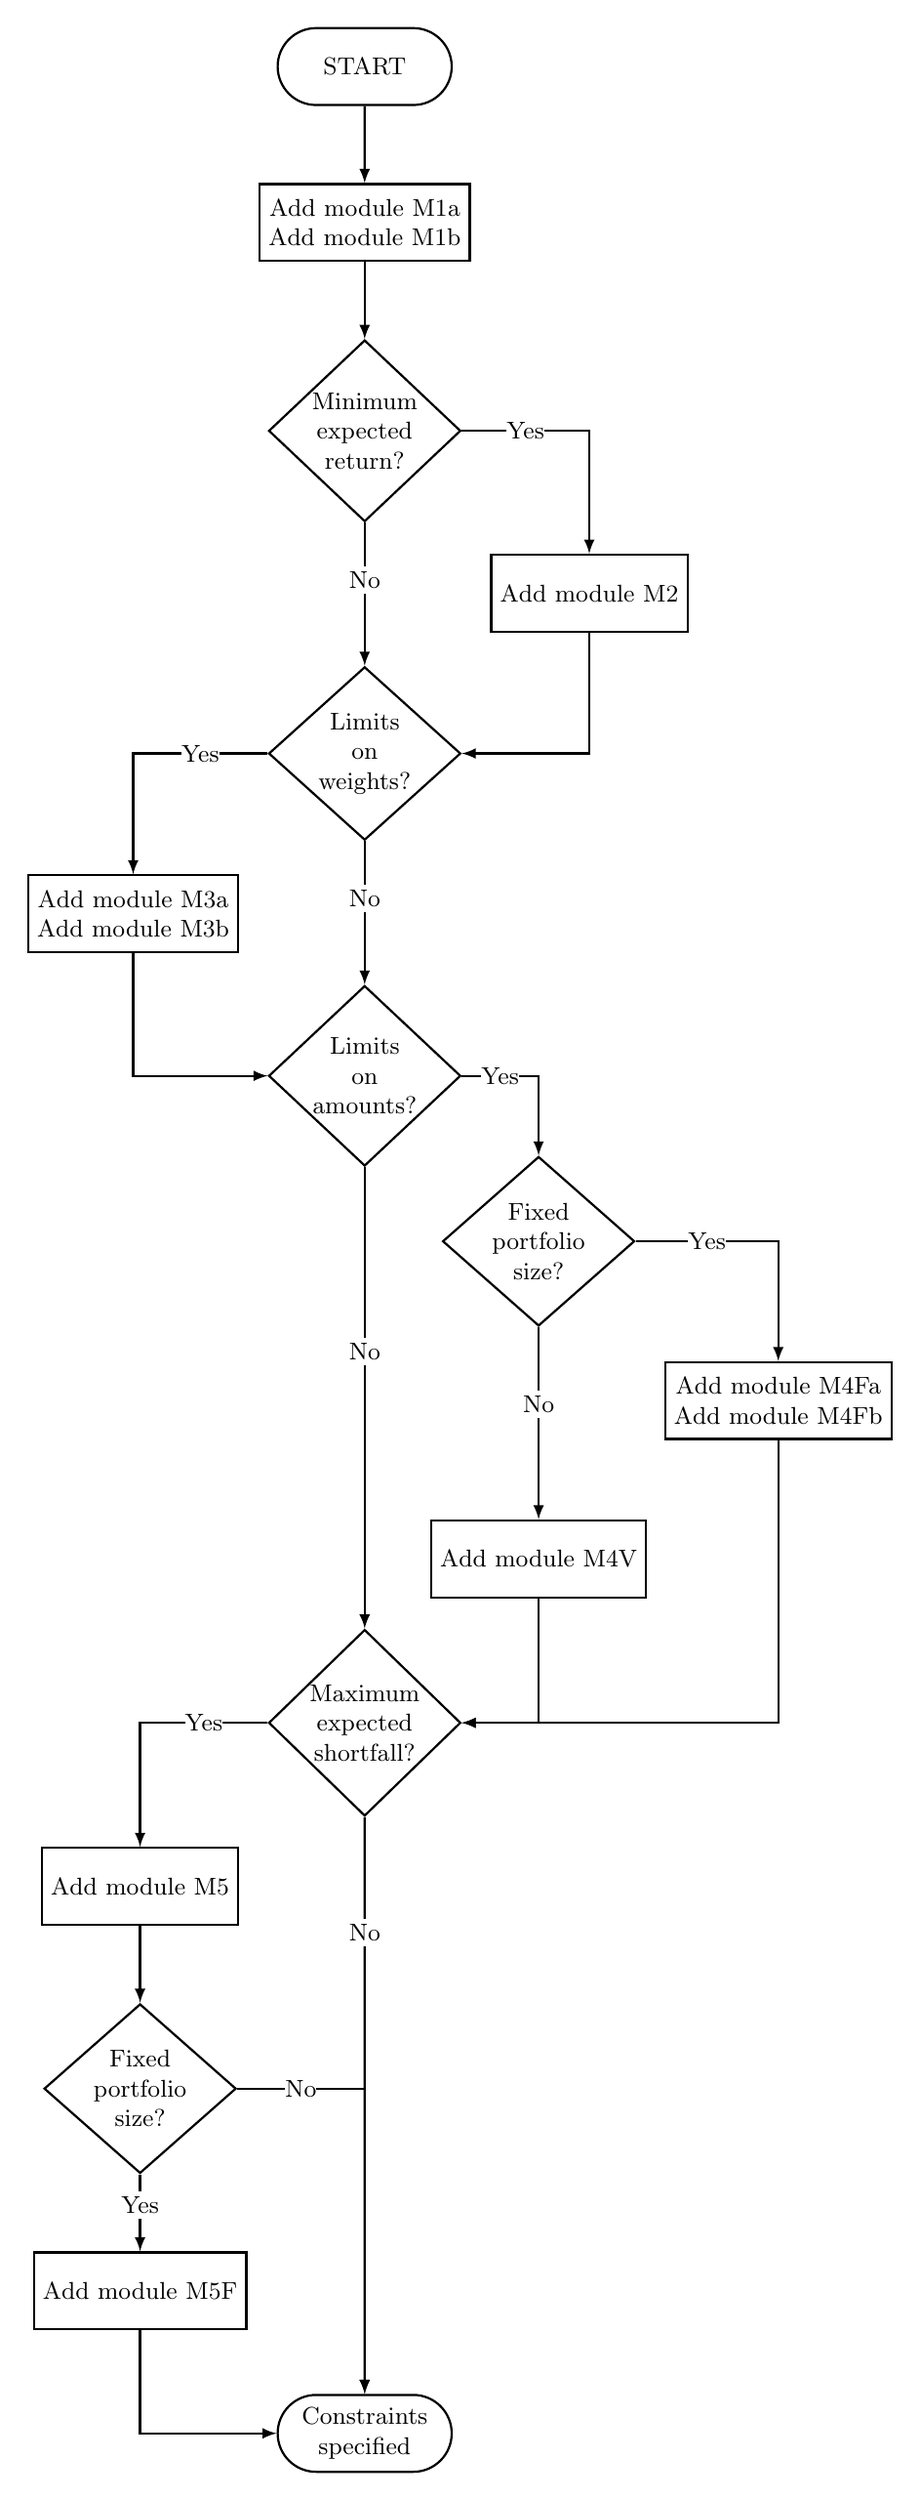
\begin{tikzpicture}[font=\small,thick]
		
		\node[draw,
		rounded rectangle,
		minimum width=2.5cm,
		minimum height=1cm] (block1) {START};
		
		\node[draw,
		align=center,
		below=of block1,
		minimum width=2.5cm,
		minimum height=1cm
		] (block3) { Add module M1a \\ Add module M1b };
		
		\node[draw,
		align=center,
		diamond,
		below=of block3,
		minimum width=2.5cm,
		inner sep=0] (block4) {Minimum \\ expected\\ return?};
		
		\node[draw,
		below right=of block4,
		minimum width=2.5cm,
		minimum height=1cm] (block5) { Add module M2};
		
		\node[draw,
		align=center,
		diamond,
		below left=of block5,
		minimum width=2.5cm,
		inner sep=0] (block6) {Limits \\ on\\ weights?};
		
		\node[draw,
		align=center,
		below left=of block6,
		minimum width=2.5cm,
		minimum height=1cm] (block7) { Add module M3a \\ Add module M3b};
		
		\node[draw,
		align=center,
		diamond,
		below right=of block7,
		minimum width=2.5cm,
		inner sep=0] (block8) {Limits \\on \\amounts?};
		
		\node[draw,
		align=center,
		diamond,
		below right=of block8,
		minimum width=2.5cm,
		inner sep=0] (block9) {Fixed \\ portfolio \\ size?};
		
		\node[draw,
		align=center,
		below right=of block9,
		minimum width=2.5cm,
		minimum height=1cm] (block10) { Add module M4Fa \\ Add module M4Fb};
		
		\node[draw,
		align=center,
		below =2.5cm of block9,
		minimum width=2.5cm,
		minimum height=1cm] (block11) { Add module M4V};
		
		\node[draw,
		align=center,
		diamond,
		below = 6cm of block8,
		minimum width=2.5cm,
		inner sep=0] (block12) {Maximum \\ expected \\ shortfall?};
		
		\node[draw,
		align=center,
		below left=of block12,
		minimum width=2.5cm,
		minimum height=1cm] (block13) { Add module M5};
		
		\node[draw,
		align=center,
		diamond,
		below =of block13,
		minimum width=2.5cm,
		inner sep=0] (block14) {Fixed \\ portfolio \\ size?};

		\node[draw,
		align=center,
		below =of block14,
		minimum width=2.5cm,
		minimum height=1cm] (block15) { Add module M5F};
		
		% Return block
		\node[draw,
		align=center,
		rounded rectangle,
		below =7.5cm of block12,
		minimum width=2.5cm,
		minimum height=1cm,] (block16) {Constraints \\specified};
		
		% Arrows
		\draw[-latex]
		(block1) edge (block3)
		(block3) edge (block4);
		
		\draw[-latex] (block4) edge
		node[pos=0.4,fill=white,inner sep=2pt]{No}(block6);
		
		\draw[-latex] (block4) -| (block5)
		node[pos=0.25,fill=white,inner sep=0]{Yes};
		
		\draw[-latex] (block5) |- (block6);
		
		\draw[-latex] (block6) -| (block7)
		node[pos=0.25,fill=white,inner sep=0]{Yes};
		
		\draw[-latex] (block6) edge
		node[pos=0.4,fill=white,inner sep=2pt]{No}(block8);
		
		\draw[-latex] (block7) |- (block8);
		
		\draw[-latex] (block8) -| (block9)
		node[pos=0.25,fill=white,inner sep=0]{Yes};
		
		\draw[-latex] (block9) -| (block10)
		node[pos=0.25,fill=white,inner sep=0]{Yes};
		
		\draw[-latex] (block8) edge
		node[pos=0.4,fill=white,inner sep=2pt]{No}(block12);
		
		\draw[-latex] (block9) edge
		node[pos=0.4,fill=white,inner sep=2pt]{No}(block11);
		
		\draw[-latex] (block10) |- (block12);
		\draw[-latex] (block11) |- (block12);
		
		\draw[-latex] (block12) -| (block13)
		node[pos=0.25,fill=white,inner sep=0]{Yes};
		
		\draw[-latex] (block12) edge
		node[pos=0.2,fill=white,inner sep=2pt]{No}(block16);
		
		\draw[-latex]
		(block13) edge (block14);
		
		\draw[-latex] (block14) edge
		node[pos=0.4,fill=white,inner sep=2pt]{Yes}(block15);
		
		\draw[-latex] (block14) -| (block16)
		node[pos=0.25,fill=white,inner sep=0]{No};
		
		\draw[-latex] (block15) |- (block16);
		
		\end{tikzpicture}
	}
	\caption{A flowchart depicting the inclusion of various portfolio constraints depending on investor preferences.}
	\label{fig:flowchart_constraints}
\end{figure}	








%
%\chapter{Technical summary}

This chapter summarizes the technical details associated with producing this report. It shows various schemas and dependencies that explain the overall structure of the whole data pipeline. Two programming languages were used for the process - R and Python. The R code is responsible for downloading the raw data, cleaning it and exporting the relevant parts. The Python code is responsible for converting the data into a lightweight format, creating and exporting the figures and compiling the final version of the report. All in all, one could say that the R part handles the data while the Python part handles the plotting and latex compilation. A visual representation of the process can be found in Figure \ref{fig:technical_summary:flowcharts_R_python}. Further details regarding specific functions and their roles can be found in tables \ref{tab:technical_summary:used_functions_R} and \ref{tab:technical_summary:used_functions_python}.

\begin{table}[h]
	\centering
	\begin{tabularx}{0.9\linewidth}{rX}
		Function name & Description \\
		\toprule
		\textbf{download\_MMSR\_data.R} & Downloads the MMSR dataset, stores it in its raw form as a large number of xml files. \\
		\textbf{redownload\_MMSR\_data.R} & A failsafe that tries to download xml files that the main download function might have missed due to connection or server issues \\
		\textbf{parse\_MMSR\_data.R} & Translates every downloaded xml file into an RData file to allow further data wrangling.  \\
		\textbf{combine\_MMSR\_data.R} & Combines the translated .RData files into monthly and yearly datasets which are in turn combined into two full datasets - one for the secured and one for the unsecured segment. Only keeps variables that are relevant for the analysis.   \\
		\textbf{prepare\_MMSR\_data.R} & Imports a full MMSR segment, removes erroneous observations, merges fixed and variable rates into a single variable, calculates maturity in business and calendar days, only keeps observations that are within the time period that we are interested in, saves the resulting dataset in multiple granularities (granular, daily, weekly, monthly) and multiple formats (.RData, .csv).\\
		\textbf{prepare\_network\_data.R} & Brackets observations by reporting agents, creates individual categories for CCPs, computes network of monthly volume exposures across pairs of agents. Creates a dataset depicting the evolution of different network centrality measures for each agent. (.RData, .csv).\\
		\textbf{functions.R} & Contains the dedicated xml parser used to translate a single xml page into an R dataframe of the correct format. \\
		\bottomrule
	\end{tabularx}
	\caption{R functions used in the analysis.}
	\label{tab:technical_summary:used_functions_R}
\end{table}

\section{Data handling}
The MMSR data is located on a dedicated server which is accessible by user's DARWIN credentials after a proper registration / data request. From this server, the data can be downloaded by directly saving an xml file with the relevant transaction details. The whole process of the data transformation within my pipeline can be seen on the left hand side of Figure \ref{fig:technical_summary:flowcharts_R_python}. I will describe the relevant steps in further detail now.

\subsection{Download}
The first step is the data download. For this purpose, we use the function \verb|download_MMSR_data.R|. This function fulfills the following tasks:
\begin{enumerate}
	\item Specifies the segment to be downloaded (secured or unsecured).
	\item Asks the user for their DARWIN credentials and stores them in a non-human-readable binary format.
	\item Creates the directory structure for the downloaded data. 
	\item Downloads the relevant xml files. Each xml file corresponds to 100 transactions on a given day, therefore the data for one day of MMSR data will likely consist of tens / hundreds of xml files. These files are saved in the created directory structure where each file's location is \ \ \verb|data/[segment]/data_raw/[year]/[month]/[day]/[page number].xml|.
	\item For each trading day, the function creates a text file that stores the total number of xml files for this particular day. The file is stored as \newline \verb|data/[segment]/data_raw/[year]/[month]/[day]/number_of_pages.txt|.
\end{enumerate}

\subsection{Download check}
In the second step, we use the function \verb|redownload_MMSR_data.R| which goes through the downloaded files and attempts to download missing data. It's possible that due to connection or server issues, some xml files have not been downloaded in the previous step. The way this function solves this issue is as follows:
\begin{enumerate}
	\item For each trading day, the function reads the file \verb|number_of_pages.txt| to determine the number of available xml files for that day $X$. If there were connection issues at this moment in the data download before, there could be further xml files for this day. Therefore, the function then attempts to download the xml file number $X+1$. If it succeeds, it continues to download further xml files at $X+2, X+3, \ldots$ until the relevant page no longer exists. In that case, it changes the value of $X$ in \verb|number_of_pages.txt| and then moves on to the next day.
	\item After checking all days in the relevant period, the function prints the number of new xml files that have been downloaded. If this number is greater than zero, it means some pages have been added which we did not have previously due to connection / server issues. It would be a good practice to run this function several times in the span of a few days to make sure there is no more data at the server. Unfortunately there is not a better way to know.
\end{enumerate}


\begin{table}[h]
	\centering
	\begin{tabularx}{0.9\linewidth}{rXc}
		\toprule
		\textbf{year} & Year of the transaction settlement  &numeric \\
		\textbf{quarter} & Quarter of the transaction settlement  &numeric\\
		\textbf{month} & Month of the transaction settlement  &numeric\\
		\textbf{week} & Week of the transaction settlement  &numeric\\
		\textbf{settlement\_date} & Day of the transaction settlement  &date\\		
		\textbf{report\_agent\_lei} & Reporting bank's unique identifier  &character\\
		\textbf{report\_agent\_loc} & Reporting bank's location code  &character\\
		\textbf{report\_agent\_name} & Reporting bank's name  &character\\
		\textbf{cntp\_sector} & Reporting bank's unique identifier  &character\\
		\textbf{cntp\_lei} & Unique identifier of the transaction counter-party  &character\\
		\textbf{cntp\_loc\_code} & Location of the transaction counter-party  &character\\
		\textbf{trns\_type} & Type of the transaction, BORR or LEND.  &character\\
		\textbf{maturity\_date} & Maturity day of the transaction  &date\\
		\textbf{trns\_nominal\_amt} & Transaction amount  &numeric\\
		\textbf{cntp\_ccp\_flag} & Binary variable that determines whether the counterparty is a central clearing party - CCP  &binary\\
		\textbf{rate} & Interest rate on the transaction p.a.  &numeric\\
		\textbf{maturity} & Number of business days until between the settlement date and the maturity date  &numeric\\
		\textbf{maturity\_calendar} & Number of calendar days until between the settlement date and the maturity date  &numeric\\
		\bottomrule
	\end{tabularx}
	\caption{Variables used in the analysis.}
	\label{tab:technical_summary:used_variables}
\end{table}

\subsection{Parsing}
In the third step, we use the function \verb|parse_MMSR_data.R|. This function leverages our parsing script from \verb|functions.R| to translate the xml files into R dataframes.
\begin{enumerate}
	\item Specifies the segment to be parsed (secured or unsecured).
	\item Specifies the sample data file to understand the data structure. This is a preemptive measure against future changes in MMSR data structure (new variables added, old variables removed etc.)
	\item Reads the xml files saved in the previous step, imports them into R, merges xml pages from the same day into a single dataframe and saves these dataframes into a new folder structure. In this new directory structure, each file is located at \newline \verb|data/[segment]/data_parsed/[year]/[month]/[day].RData|.
\end{enumerate}

\subsection{Merging}
In the fourth step, we use the function \verb|combine_MMSR_data.R|. This function combines the dataframes into chunks of monthly and yearly datasets, also creating one single dataframe for each segment.
\begin{enumerate}
	\item Specifies the segment to be merged (secured or unsecured).
	\item Specifies the variables relevant for the analysis and this report and drops the rest. Variables that are being kept can be found in Table \ref{tab:technical_summary:used_variables}.
	\item Goes through all saved dataframes and creates a new directory structure with merged data. In this new directory structure, each file with monthly data is located at \newline \verb|data/[segment]/data_combined/[year]/[month].RData|. There are also yearly data files located at \verb|data/[segment]/data_combined/[year].RData| and a master dataframe for each segment located at \verb|data/[segment]/data_combined/merged_df.RData|.
\end{enumerate}




\subsection{Cleaning}
In the fifth step, we use the function \verb|prepare_MMSR_data.R|. This function takes care of cleaning the data and producing a dataset with different granularities.
\begin{enumerate}
	\item Specifies the segment to be handled (secured or unsecured).
	\item Loads the merged dataframe located at \verb|data/[segment]/data_combined/merged_df.RData|.
	\item Specifies which variables are supposed to be numeric and converts them into their correct numeric format.
	\item Drops novations and invalid observations.
	\item Coverts the variables representing the fixed interest rate and the variables representing the variable interest rate into a single variable called \verb|rate|.
	\item Converts the settlement and maturity dates into their correct format, creates new variables called (\verb|maturity|) \verb|maturity_calendar| which contain the number of (business) days until the transaction matures.
	\item Remove the data before 2017Jan01 and after the last month's end.
	\item Merges the data appropriately to not only create the full granular transaction-level dataset, but also daily, weekly and monthly datasets. Additional datasets are created where only observations from a particular bank or country are included. Each of these datasets is stored both as an R dataframe as well as a csv file.
	\item Creates a new directory structure where these datasets are stored within \newline \verb|data/[segment]/data_prepared/|.
\end{enumerate}



\begin{figure}[H]
	\centering
	\begin{subfigure}{.5\textwidth}
		\centering
		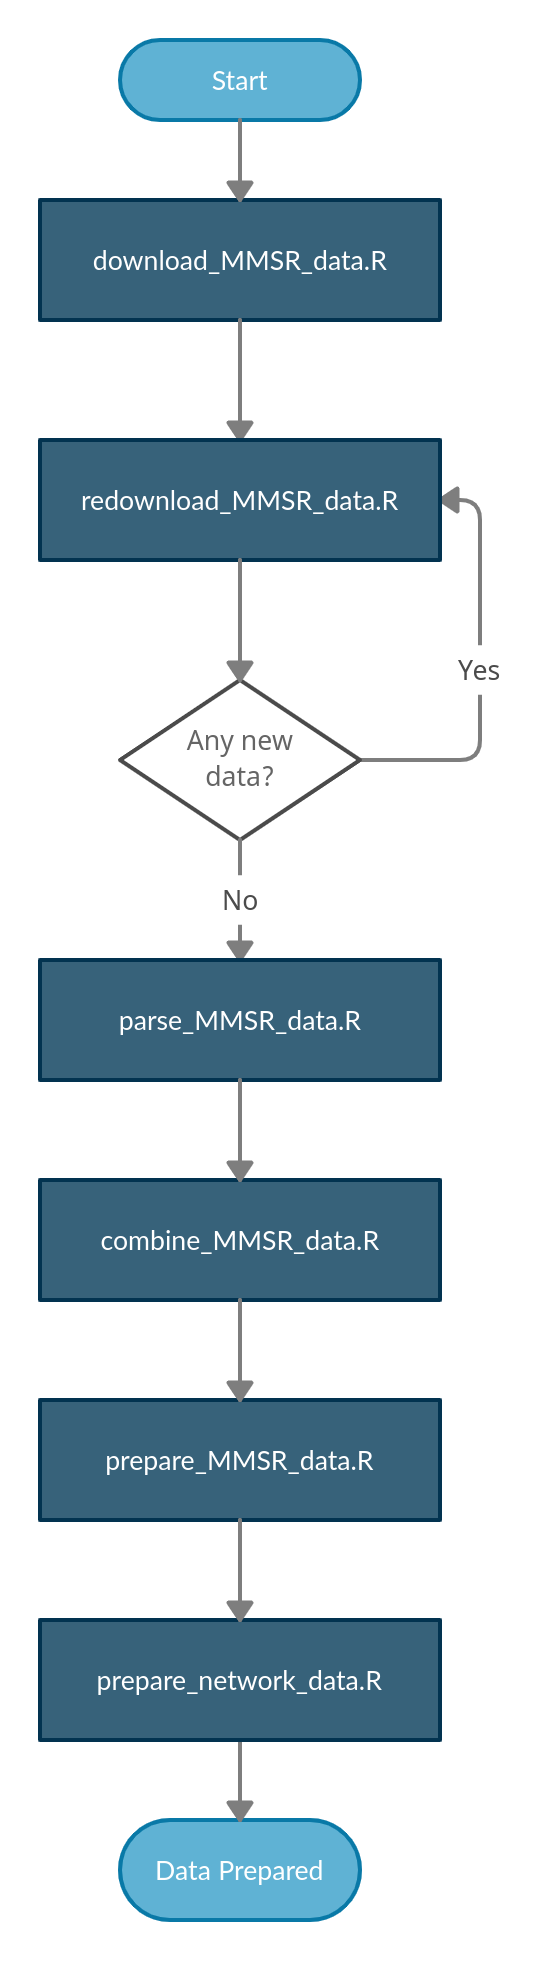
\includegraphics[width=0.75\textwidth]{\detokenize{figures/flowchart_R}}
		\vspace{12pt}
		\caption{The part of the pipeline responsible for downloading, parsing, combining and cleaning the data. Coded in R.}
	\end{subfigure}%
	\begin{subfigure}{.5\textwidth}
		\centering
		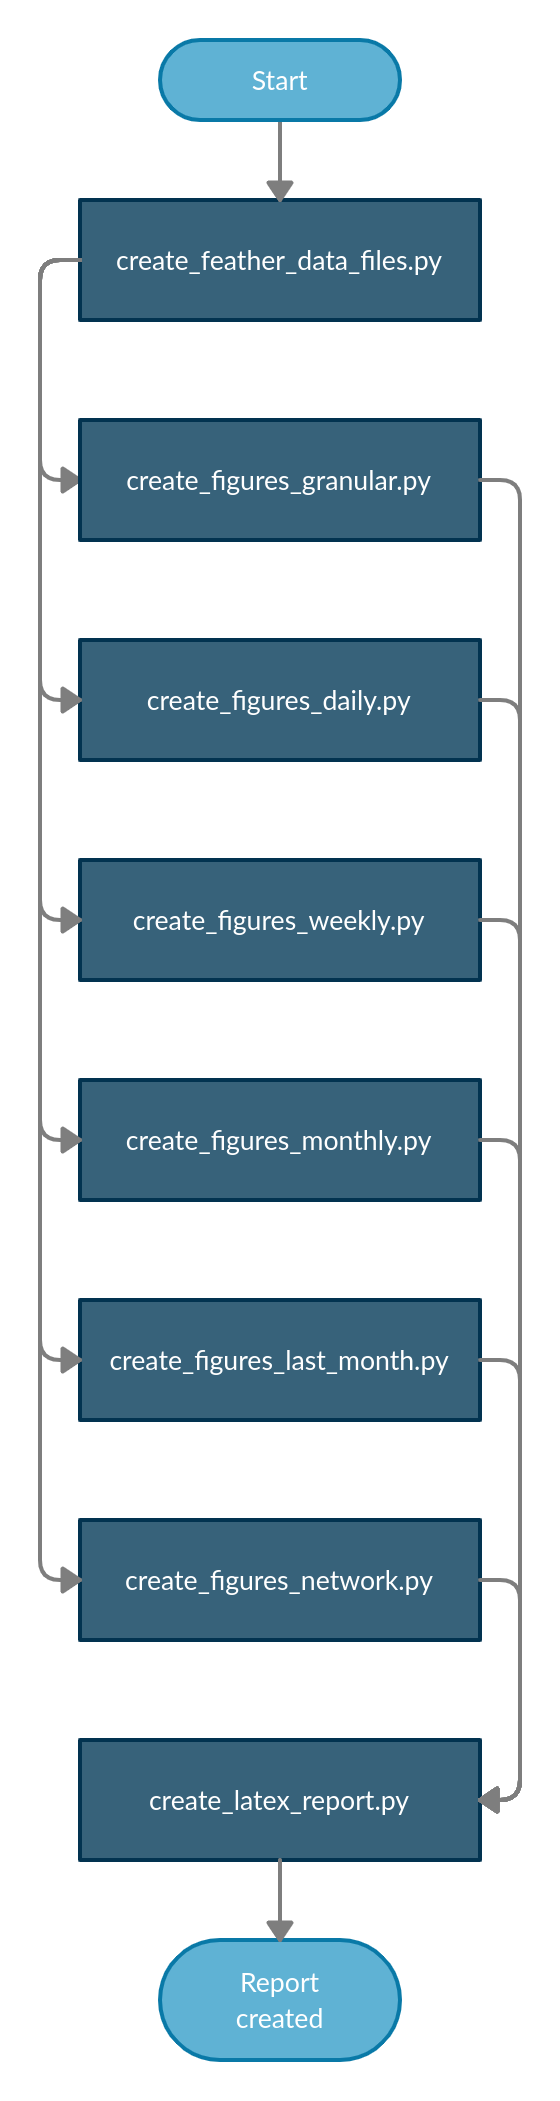
\includegraphics[width=0.735\textwidth]{\detokenize{figures/flowchart_python}}
		\caption{The part of the pipeline responsible for creating lightweight data files, plotting figures and compiling this final pdf report. Coded in Python.}
	\end{subfigure}
	\caption{Graphical visualization of the whole pipeline.}
	\label{fig:technical_summary:flowcharts_R_python}
\end{figure}



\section{Plotting and report compilation}

The figures in this report have been plotted by the python part of the pipeline. The relevant process can be seen on the right hand side of Figure \ref{fig:technical_summary:flowcharts_R_python} while Table \ref{tab:technical_summary:used_functions_python} contains short descriptions of each python function used. I will now describe the process in further detail.


\begin{table}[h]
	\centering
	\begin{tabularx}{0.9\linewidth}{rX}
		Function name & Description \\
		\toprule
		\textbf{create\_feather\_data\_files.py} & Loads the created .csv files, creates new temporal variables, saves different datasets under different granularities. \\
		\textbf{create\_figures\_granular.py} & Creates multiple figures using the full granular dataset.  \\
		\textbf{create\_figures\_daily.py} & Creates multiple figures using the daily dataset.\\
		\textbf{create\_figures\_weekly.py} & Creates multiple figures using the weekly dataset.\\
		\textbf{create\_figures\_monthly.py} & Creates multiple figures using the monthly dataset.\\
		\textbf{create\_figures\_last\_month.py} & Creates multiple figures using the granular dataset containing the last month's transactions.\\
		\textbf{create\_figures\_network.py} & Creates multiple figures using the prepared network centrality dataset.\\
		\textbf{create\_latex\_report.py} & Creates and compiles the final MMSR monthly pdf report.\\
		\textbf{plotting\_functions.py} & Contains definitions and settings of all functions used for figure plotting. \\
		\textbf{config.py} & Contains global variables that are unchanged during the execution of the script such as the root folder path etc.\\
		\bottomrule
	\end{tabularx}
	\caption{Python functions used in the analysis.}
	\label{tab:technical_summary:used_functions_python}
\end{table}

\subsection{Feather data files}
In the first step of this part, we convert the datasets exported with R into a feather file format. The feather file format is a special way of storing data that allows for extremely fast loading / saving. It considerably speeds up our  next computations. For this purpose we use the function \verb|create_feather_data_files.py|. This function:
\begin{itemize}
	\item Loads the relevant granular, daily, weekly and monthly datasets from csv files.
	\item Creates new variables relevant for figure plotting such as year+month, year+quarter etc.
	\item Saves the new files as feather dataframes within a newly created directory structure at:\newline\verb|data/[segment]/data_feather/|.
\end{itemize}

\subsection{Plotting}
In the second step, we use several functions to plot our data. The core of the plotting is coded within the \verb|plotting_functions.py| function and almost in all cases leverages the \verb|seaborn| library. Various different scripts then use these low-level plotting functions to achieve a consistent look of the whole document. These include:
\begin{itemize}
	\item \verb|create_figures_granular.py| - this function leverages the full transaction-level data and produces the associated figures where such transaction-level data is necessary. For instance, all heatmap figures where dependencies between pairs of variables need to be studied are compiled with this function.
	\item \verb|create_figures_daily.py| - this function plots figures where looking at daily quantities is sufficient such as daily volumes, rates and maturities.
	\item \verb|create_figures_weekly.py| - this function plots figures where looking at weekly quantities is sufficient such as daily volumes, rates and maturities.
	\item \verb|create_figures_monthly.py| - this function plots figures where looking at monthly quantities is sufficient such as daily volumes, rates and maturities.
	\item \verb|create_figures_last_month.py| - this function again leverages the full transaction-level data and produces the associated figures where such transaction-level data is necessary. but only for the last month's data. It is used to create figures for chapters summarizing the last month in data.
	\item \verb|create_figures_network.py| - this function plots the figures associated with the network analysis.
\end{itemize}

\subsection{Report compilation}
The third and final step of data visualization entails formatting of this report. I use the \verb|pylatex| python library which allows me to algorithmically generate a latex report and compile via a Python interface. Only the short \verb|report.tex| file within the \verb|/report/| is algorithmically generated, any further chapters and dependencies are fixed and handled with the latex code.


\section{Installation}
Various software and software packages are required to install dependencies for this pipeline. I have strived to make this list of prerequisites as complete as possible but it's very likely there are further steps required that I have forgotten to include.
\begin{itemize}
	\item install RStudio and R
	\item R prompt: install.packages('bizdays')
	\item R prompt: install.packages("readstata13")	
	\item R prompt: install.packages("sqldf")
	\item R prompt: install.packages("XML")
	\item R prompt: install.packages("xml2")	
	\item R prompt: install.packages("httr")
	\item R prompt: install.packages("getPass")
	\item install Anaconda for python
	\item reinstall MikTex
	\item install latexmk package through miktex console
	\item install ActivePerl through the OeppStore
	\item conda prompt: pip install pylatex
	\item conda prompt: pip3 install pandasql
	\item conda prompt: pip3 install pyreadr
	\item conda prompt: pip3 install seaborn==0.11.0
\end{itemize}
%
\bibliographystyle{plainnat}
\bibliography{literature}

\appendix%

\end{document}